\section{Durchführung}
Bevor wir mit der Aufnahme der Messdaten beginnen, machen wir noch einige theoretische Vorüberlegungen:
\subsection{Radon-Transformation als Rekonstruktionsverfahren: Ein Rechenbeispiel} \label{dfs:Radon}
        Im Folgenden soll die durch die Auswertungssoftware durchgeführte (diskrete) Radon-Transformation anhand einer willkürlich gewählten Aktivitätsverteilung $N(x,y)$ nachvollziehbar dargestellt werden. Da der Ort $(x,y)$ technisch nicht als kontinuierliche Variable implementiert werden kann, genügt die Betrachtung der Ausgangsverteilung als eine Matrix $\boldsymbol{I} \in \mathbb{R}^{5 \times 5}$ mit endlichen Dimensionen, deren Einträge die Aktivität am jeweiligen Ort repräsentieren. Zunächst bestimmt man das sogenannte \textbf{Sinogramm} $p(s, \theta)$, indem man das Koordinatensystem um einen Winkel $\theta$ dreht und dann die Verteilung $N(x'(s,\theta),y'(s,\theta))$ zu einem bestimmten Ort s, welcher ohne Beschränkung der Allgemeinheit mit der x-Koordinate des gedrehten Systems identifiziert werden kann, entlang der neuen y-Achse integriert. Was wir erhalten, ist eine Projektion der Ausgangsverteilung auf die gedrehte x-Achse. Diese Konstruktion wirkt künstlich, ist aber letztlich genau das, was bei einem PET-Scan geschieht: Rotiert man die Detektoren um eine Quelle, so misst man für jeden festen Winkel genau die oben beschriebene Projektion der Quellverteilung auf die Detektorfläche.\\
        \ \\
         Numerisch simulieren wir diese Hin-Transformation dadurch, dass über die einzelnen Einträge in den Spalten ($\theta = 0\ \unit{°}$), den Zeilen ($\theta = 90\ \unit{°}$) und den Diagonalen ($\theta = 90\ \unit{°},\ 135\ \unit{°}$) von $\boldsymbol{I}$ summiert wird. Da die Matrix 9 Diagonalen besitzt, sie allerdings analog zu den Zeilen und Spalten in 5 Teile 'zerschnitten' werden müsste, müssen die so erhaltenen Diagonalsummen $\boldsymbol{D} \in \mathbb{R}^{1 \times 9}$  durch Multiplikation einer Wichtungsmatrix $\boldsymbol{W_{Proj}} \in \mathbb{R}^{9 \times 5}$ multipliziert werden, um die unterschiedlichen 'Flächenanteile' der Diagonalen an der 'Gesamtfläche' der Matrix zu berücksichtigen. Dadurch wird das Sinogramm insgesamt zu einer Matrix $\boldsymbol{P} \in \mathbb{R}^{4 \times 5}$, deren Zeilen die Variation des Winkels $\theta$ und deren Spalten die Änderung des Ortes $s$ repräsentieren.\\
        \ \\
        Nach erfolgreicher Hintransformation wird nun der Einfluss eines \textbf{Ramp-Filters} untersucht. Dieser Filter wird durch eine Filterfunktion $h(s)$ modelliert, die folgenden Eigenschaften genügt:
        \begin{itemize}
        		\item[(i)] $\lim\limits_{s\rightarrow 0}h(s) = \infty$
        		\item[(ii)] $\lim\limits_{|s|\rightarrow \infty}h(s) = 0$
        		\item[(iii)] $\forall s \in \mathbb{R}\setminus\{0\}:\ h(s) < 0$
        		\item[(iv)] $h$ ist symmetrisch
        \end{itemize}
        Man findet folgenden formalen analytischen Ausdruck für h\cite{Ramp}
        
        \begin{equation*}
        	h(s) = \begin{cases}
        				- \frac{1}{2 \pi^2 s^2} & s \neq 0\\
        				\frac{\delta(s)}{\pi^2 |s|} & s = 0\\
        			\end{cases}
        \end{equation*}\\
        Damit erhält man das gefilterte Sinogramm $p_f(s,\theta)$ durch die Faltung der Filterfunktion mit dem ermittelten Sinogramm:
        \begin{equation}\label{dfe:Faltung}
                	p_f(s,\theta) := (p(\cdot, \theta) \ast h) (s) = \int_{-\infty}^{\infty}  p(s', \theta) \cdot h(s-s') \mathrm{d}s'
        \end{equation}\\
        Da die mathematischen Objekte im vorliegenden Fall von diskreter Natur sind, wird die Filterfunktion durch einen Vektor:
        \begin{equation*}
        		\boldsymbol{H} = (0, \dots , 0, -b_d,-b_{d-1}, \dots, -b_1,a,-b_1, \dots, -b_{d-1}, -b_d,0, \dots, 0) \in \mathbb{R}^{5 \times 1},\ \forall j = 1,\dots, d: b_j, a > 0
        \end{equation*}\\  
        modelliert, der offenbar den Eigenschaften (ii) - (iv) genügt. Dabei wird $d$ die \textbf{Dimension} des Filters genannt, die anschaulich angibt, wie viele linke und rechte Nachbarn eines Eintrages der Sinogrammmatrix man zu diesem gewichtet dazuaddiert. Diese Operation entspricht der Faltung in (\ref{dfe:Faltung}) und kann durch eine geeignete Matrixmultiplikation von $\boldsymbol{P}$ mit $\boldsymbol{H}$  dargestellt werden. Wobei $\boldsymbol{P}$ noch mit $d$ Nullspalten links und rechts erweitert werden muss (analog $\boldsymbol{H}$), damit die Einträge am Rand der Matrix 'Nullnachbarn' erhalten. Das liefert uns die gefilterte Matrix $\boldsymbol{P_f} \in \mathbb{R}^{4\times 5}$.\\
        \ \\
        Nach der Filterprozedur wird jetzt die inverse Transformation durchgeführt. Das heißt, man iteriere jetzt durch die Zeilen von $\boldsymbol{P}$ bzw. $\boldsymbol{P_f}$, die die Sinogrammwerte zu den verschiedenen Winkeln $\theta$ repräsentieren, und verteile diese gleichmäßig(!) auf die Zeilen, Spalten und Diagonalen. Erneut sind die Diagonalen gesondert zu behandeln, indem man die betreffenden Zeilen mit einer Wichtungsmatrix $\boldsymbol{W_{InvProj}} \in \mathbb{R}^{5 \times 9}$ multipliziert. Die Rückprojektion erhält man nun durch Addition der so entstandenen 4 Matrizen, wobei die Diagonalmatrizen nur mit einem Wichtungsfaktor von $0,5$ eingehen. Das Ergebnis der gefilterten und ungefilterten Rückprojektion anhand eines vorgegebenen Beispiels mit einem Rampfilter der Dimension $d=1$ wird im Folgenden dargestellt:\\
        \begin{tabular}{p{5.3cm}p{5.3cm}p{5.3cm}}
                	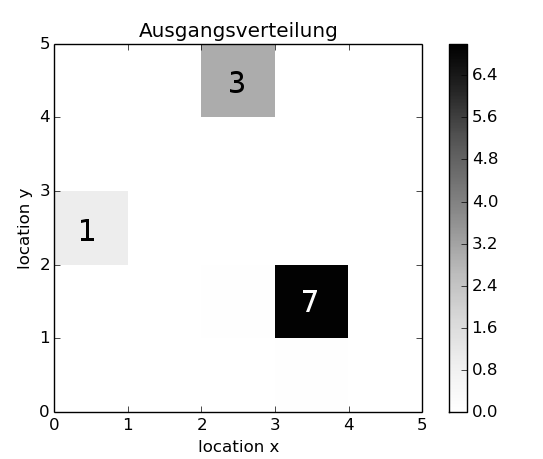
\includegraphics[width=0.36\textwidth, height=0.2\textheight]{pic/radonInp.png}
                    & 
                    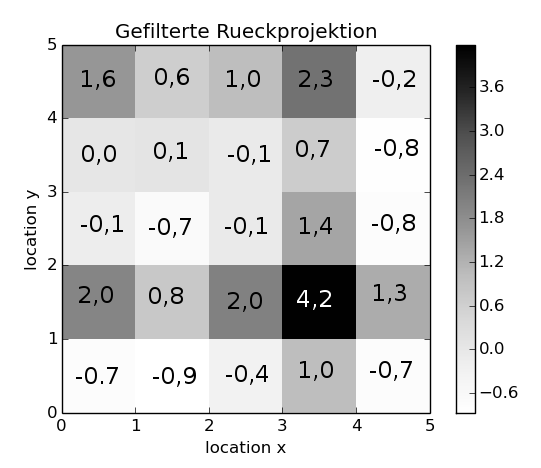
\includegraphics[width=0.36\textwidth, height=0.2\textheight]{pic/radonGef.png}
                    &
                  	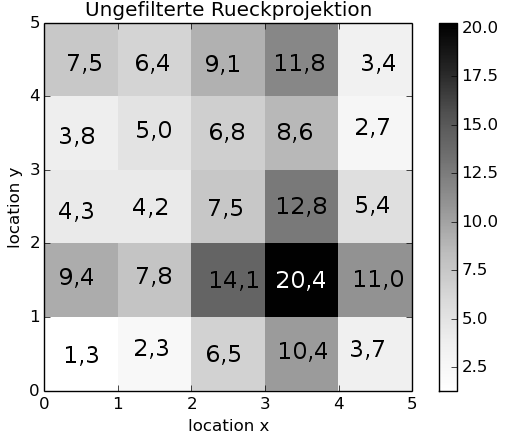
\includegraphics[width=0.355\textwidth, height=0.19\textheight]{pic/radonUngef.png}                                     
         \end{tabular}
         \captionof{figure}{Theoretisches Beispiel für Radon-Transformation}
         \label{dfd:Radon}
         \vspace{3mm}  
        
        Die Berechnung und Darstellung erfolgte über ein selbst geschriebenes \texttt{python}-Skript, das den oben beschriebenen Algorithmus realisiert. Wir sehen, dass trotz der Einfachheit des Beispiels enorme Abweichungen zwischen Ausgangsverteilung und Rückprojektion entstehen: Bis auf den größten Peak bei $(x = 3,\ y = 1)$ alle Maxima leicht versetzt rückprojiziert wurden. Dies liegt zum einen an der Diskretisierung des Problems und zum anderen besitzt selbst die über das Fourier-Scheiben-Theorem durchgeführte Rücktransformation keine exakte Lösung, da ein divergentes Integral darin auftritt, das auf einen endlichen Integrationsbereich heruntergebrochen werden muss.\cite{PA} Der Ramp-Filter führt dazu, dass die Peaks schneller abfallen und somit besser lokalisiert werden können, was sich bei der späteren quantitativen Auswertung noch als nützlich erweisen wird.

\subsection{Kalibriermessungen}
Bevor die eigentlichen Messdaten aufgenommen werden können, muss die Messapperatur kalibriert werden:
    \subsubsection{Messung einer Quelle bekannter Aktivität bei mittiger Quellposition} \label{dft:kalib_mitte}
       Zunächst haben wir eine Quelle in mittigem Abstand zu den beiden Detektoren vermessen. Die Quelle hatte am 29.10.2015 eine Aktivitiät $A = \unit[1,02]{MBq}$.\\
       Daraus sollten die Energiefenster der beiden Detektoren sowie das Koinzidenzzeitfenster bestimmt werden. Die Energiepeaks werden um $\unit[511]{keV}$ erwartet, was einem
       Kanal von 2402 für Detektor A und 1868 für Detektor B entspricht. Das Zeitfenster erwarten wir aufgrund technischer Effekte (bspw. Totzeit) und einer gewollten
       erhöhten Verzögerung im Bereich einiger zehn Nanosekunden.  
       \vspace{2mm}
        
       \begin{longtable}{p{6cm}p{6cm}l}
               \minipanf 
                   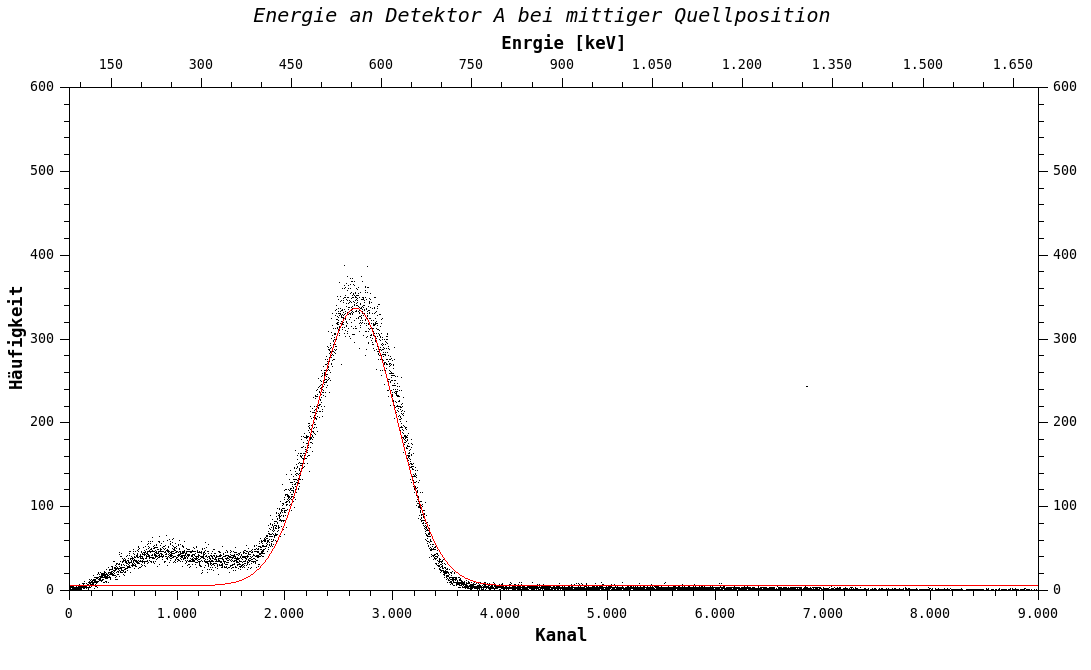
\includegraphics[width=1.2\textwidth, height=0.225\textheight]{pic/Efenster_DetA_M.png}
                   \label{dfd:EdetA_M}
               \minipend
               &
               \hspace{9mm}
               \minipanf 
                   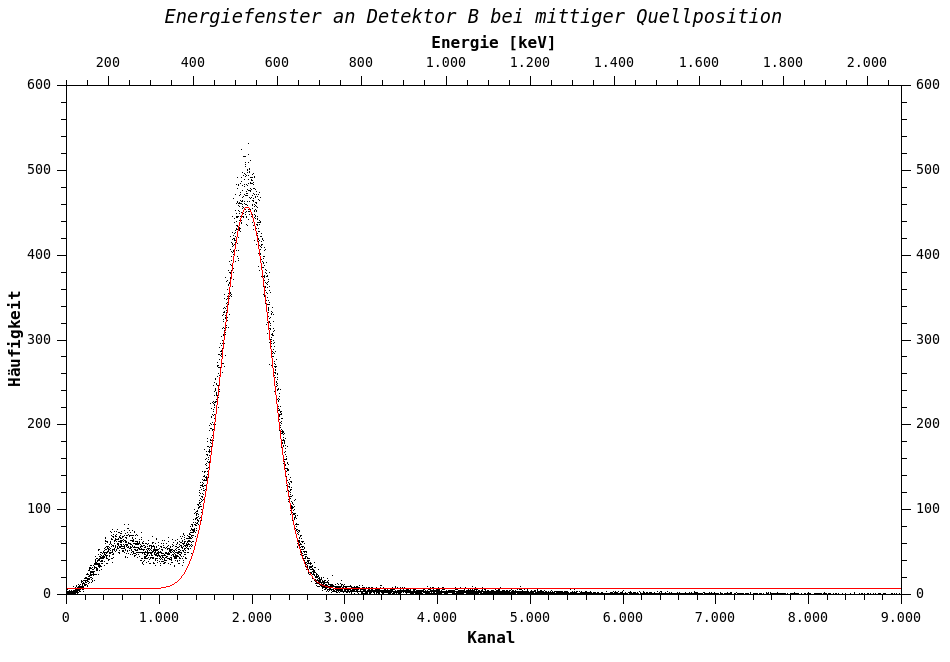
\includegraphics[width=1.2\textwidth, height=0.225\textheight]{pic/Efenster_DetB_M.png}
                   \label{dfd:EdetB_M}
               \minipend\\
               \multicolumn{2}{c}{\hspace{1.5cm}
                   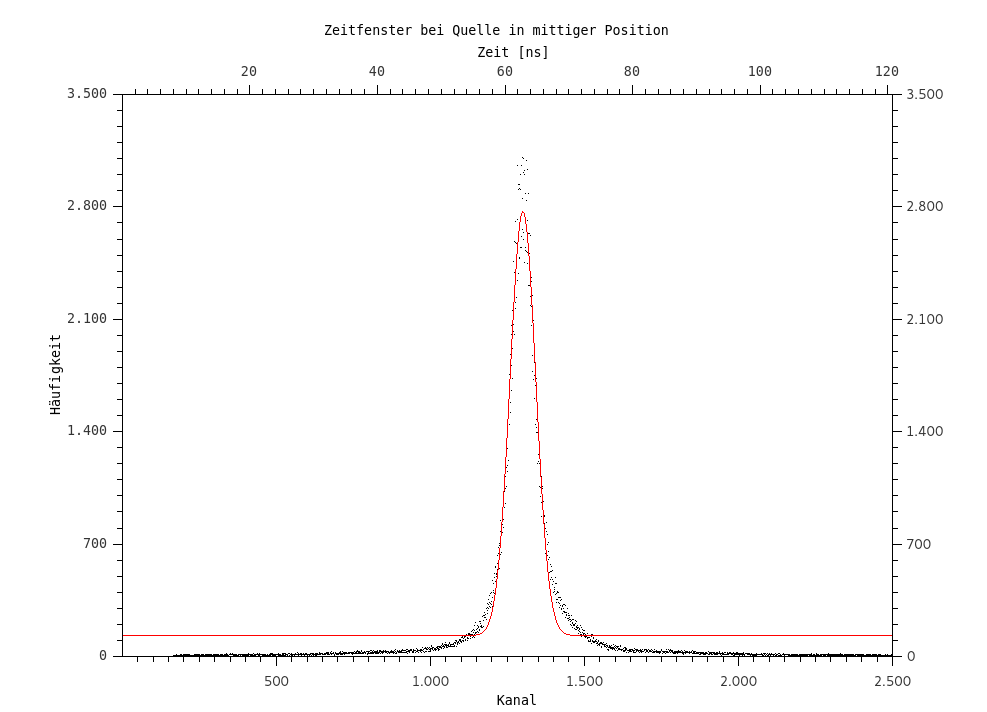
\includegraphics[width=0.7\textwidth, height=0.3\textheight]{pic/T_M_dia.png}
                   \label{dfd:T_M}}\\                        
       \end{longtable}
       \captionof{table}{Kalibrationsmessung bei Quelle mittig zwischen den Detektoren A und B}
       \label{dft:kalim}
       \ \\
       Wie man an den oberen beiden Diagrammen von Tabelle \ref{dft:kalim} sieht, stimmt diese Erwartung mit einer leichten Verschiebung nach rechts gut überein. Dies kann
       dem statistischen Charakter von Kernzerfällen und den Wegen (verändert ua. durch Compton-Streuung für Photonen, freiwerdende Bremsstrahlung für Positronen), die die 
       Positronen und letztlich die Photonen zurücklegen zugeordnet werden. Andererseits unterliegen die Detektormessungen und die Umrechnung der Kanäle in Energien einem 
       Fehler, da die Kanäle diskret sind und nur bestimmte Energien detektieren können, was dazu führt, dass Energien zwischen zwei Kanälen verloren gehen.
       Die Umrechnung der Kanäle in Energien und Zeit erfolgt mittels folgender, uns gegebener Formeln des Musters $G = a + b \cdot K$, wobei K die Kanalnummer meint und a
       bzw. b Parameter sind:
       \begin{gather*}
           E_A = (81\pm 31) + (0,179\pm 0,012)K_A\\
           E_B = (100\pm 40) + (0,220\pm 0,021)K_B\\
           \Delta t = (-0,014\pm 0,0192) + (0,0483\pm 0,00002)K_t
       \end{gather*}
       
       Die Fehler für die Umrechnung von Kanälen in physikalische Einheiten lassen sich leicht über die gauß'sche Fehlerfortpflanzung bestimmten und belaufen sich betreffend 
       der Diagramme in \ref{dft:kalim} auf:\\
       $$ \Delta(\Delta t) = \unit[0,03]{ns} ; \Delta E_A = \unit[44,84]{keV}; \Delta E_A = \unit[44,00]{keV} $$
       Um Messungen vorzunehmen, müssen jetzt die Fenster für Energie und Koninzidenzzeit bestimmt werden. Dies geschieht über Gauß-Fits in den Diagrammen von Tabelle \ref{dft:kalim}.
       Dann bestimmt man das FWHM und zieht es von den Maxmumpositionen ab. Damit ergeben sich die Fenster zu:
       $$ K_A \in \left[ 2217, 3101\right], K_B \in \left[ 1629, 2264 \right],  K_t \in \left[1252, 1351\right] $$ 
       $$ E_A \in \left[478 , 636\right] \unit{keV}, E_B \in \left[ 458, 598\right] \unit{keV},  \Delta t \in \left[60, 65\right]\unit{ns} $$ 
       Daraus ergibt sich eine Koinzidenzauflösungszeit von $\tau = \unit[(4,77 \pm 0,02)]{ns}$, welche auf eine Abschätzung der zufälligen Koinzidenzen führt. Mithilfe der gegebenen Positronenemissionswahrscheinlichkeit
       für $\unit[^{22}]{Na}$ können wir die Zahl der Zerfälle berechnen, die keine Positronen emittieren. Im schlimmsten Fall würden alle diese Zerfälle einen Beitrag zufälliger Koinzidenzen beisteuern, was 
       zehn Prozent der gemessenen Ereignisse ausmacht. Bei $\unit[^{22}]{Na}$ bestehen diese restlichen Prozesse aus $\gamma\unit{-Quanten}$ mit einer Energie von 1275 keV. Diese kann man vor allem in den späteren
       Messungen, die direkt an den Detektoren gemacht wurden, erkennen. (Siehe Abbildung \ref{dft:kaliAB}) Einen Großteil dieser Ereignisse schließen wir jedoch durch die Kalibrierung und die Setzung der Zeitfenster
       aus, sodass der Einfluss keine 10\% mehr ausmacht. Deshalb ist die Zahl der zufälligen Koinzidenzen besser abschätzbar über die Standardabweichung im Zusammenhang mit dem Anteil der Prozesse, die beim Zerfall 
       keine Positronen emittieren. Hierfür ergibt sich die Zahl der zufälligen Koinzidenzen zu $N = 147$.\\
       
       \textbf{Koinzidenznachweiseffektivität}\\
       Mit diesen Informationen lassen sich nun die Koinzidenznachweiseffektivitätem der verwendeten Detektoren A und B berechnen. Gegeben sind zunächst folgende Formeln für die Zählrate wahrer Koinzidenzen:
       \begin{gather}
           \dot N_K = \left( \frac{\Omega _{min}}{2\pi} \right) A P_\beta \varepsilon_A \varepsilon_B
           \label{dff:NK}\\
           \dot N_Z = \left( \frac{2\tau A\Omega _{min}}{\pi} \right)\dot N_K
           \label{dff:NZ}
       \end{gather}
       
       Dabei sind $\varepsilon_{A/B}$ die Nachweiseffektivitäten der Detektoren, $P_\beta$ die Positronenemissionswahrscheinlichkeit und $\Omega_{min}$ der Raumwinkel des Detektors, der am weitesten von der Quelle entfernt
       ist. $\dot N_Z$ ist die Zählrate zufälliger Koinzidenzen. Setzt man die Gleichungen \ref{dff:NK} und \ref{dff:NZ} ineinander ein, erhält man folgende Gleichung für die Nachweiseffektivitäten:
       $$ \varepsilon_A \varepsilon_B = \frac{\pi^2 \dot N_Z}{A^2 P_\beta \tau \Omega^2_{min}} \text{ mit } \Omega_{min} = \frac{4a}{\left(D-b\right)^2 } \text{ und } \dot N_Z = \frac{N_Z}{\tilde t}$$
       Da die Nachweiseffektivität pro Detektor zu bestimmen ist, kann man $ \varepsilon_A \simeq \varepsilon_B $ annehmen und erhält:
       $$ \varepsilon_{A/B} = \sqrt{\frac{\pi^2 N_Z}{A^2 \Omega^2_{min} P_\beta \tau \tilde t_{A/B}}}$$ 
       Für den Fehler erhält man bei fehlerlos angenommenen b, D, und a folgendes:
       $$ \Delta\varepsilon_{A/B} = \varepsilon_{A/B} \cdot\sqrt{\left(\frac{\Delta P_\beta}{P_\beta}\right)^2+ \left(\frac{2\Delta A}{A}\right)^2 + \left(\frac{\Delta \tau}{\tau}\right)^2+ \left(\frac{\Delta \tilde t_{A/B}}{\tilde t_{A/B}}\right)^2}$$
       Die verwendeten Daten sind folgende:
       $$ D = \unit[386]{mm}, b = \unit[25]{mm}, a = \unit[54]{mm}, P_\beta = 0,90382 \pm 0,00021, \tilde t_B = \unit[(230 \pm 0,1)]{s} , \tilde t_A = \unit[(314\pm7)]{s}$$
       Damit erhalten wir für die Detektoren folgende Nachweiseffektivitäten:
       $$ \varepsilon_A = \unit[(46\pm 3)]{\%}, \varepsilon_B = \unit[(54\pm 3)]{\%}$$
       Diese Nachweiseffektivität ist für einen Versuchsplatz angemessen gut, im Vergleich zu in Krankenhäusern verwendeten Geräten, welche mit einer Effektivität von 80\% arbeiten.

    \subsubsection{Messung bei Positionen direkt an den Detektoren}
        Als nächstes soll der Abstand der beiden Detektoren zueinander bestimmt werden. Hierfür erfolgen Messungen, bei denen die Kalibrierquelle direkt an den Detektoren positioniert wird.
        Wie oben angedeutet, sieht man in den nachfolgenden Diagramme auch die Detektionen von den Photenen der Zerfallsreihe mit nur 10\% Wahrscheinlichkeit, eben jenen Prozessen, die nicht
        die gewollte Positronenemission erzeugen. Besonders gut fällt dies dort auf, wo die Quelle wirklich direkt am Detektor liegt nicht und nicht am gegenüberliegenden.
        Am gegenüberliegenden Detektor sieht man jeweils zwei große Peaks von denen einer im niedrigeren Energiebereich als dem erwarteten liegen.
        Dies ist auch nachvollziehbar, da alle gestreuten und durch Bremsstrahlung erzeugten Photonen mitgezählt werden.
        \begin{longtable}{p{6cm}p{6cm}l}
            \minipanf 
                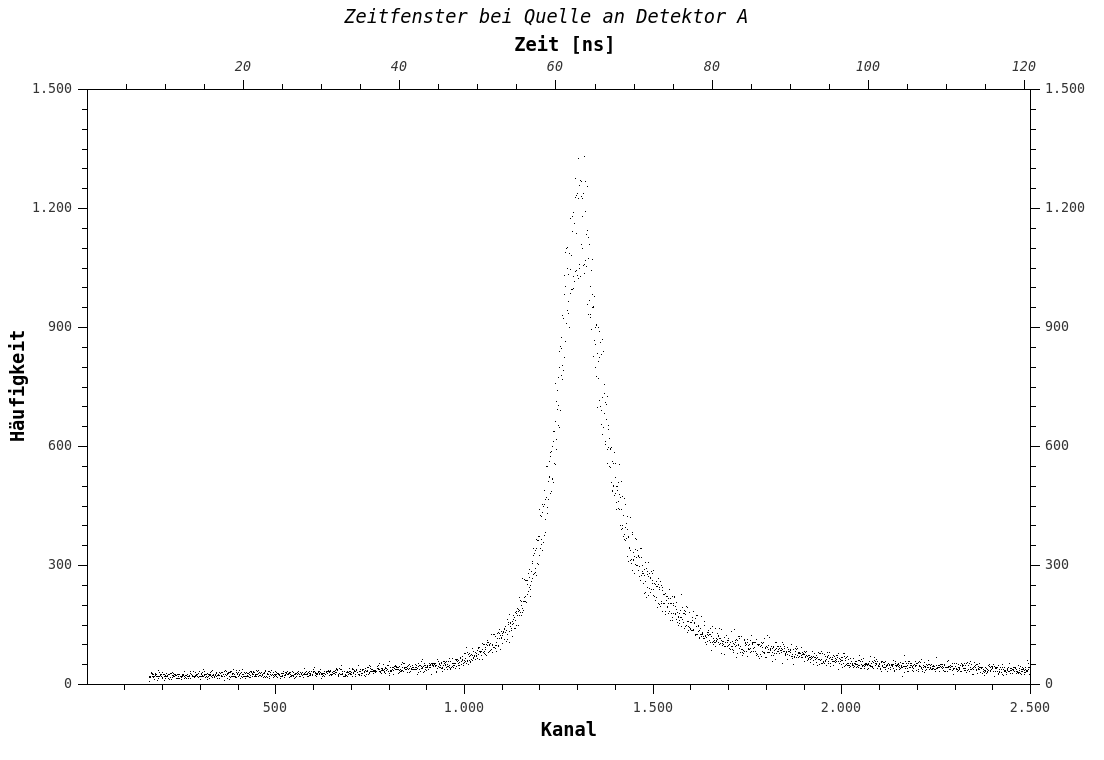
\includegraphics[width=1.2\textwidth, height=0.225\textheight]{pic/T_A_dia.png}
                \label{dfd:T_A}
            \minipend
            &
            \hspace{9mm} 
            \minipanf
                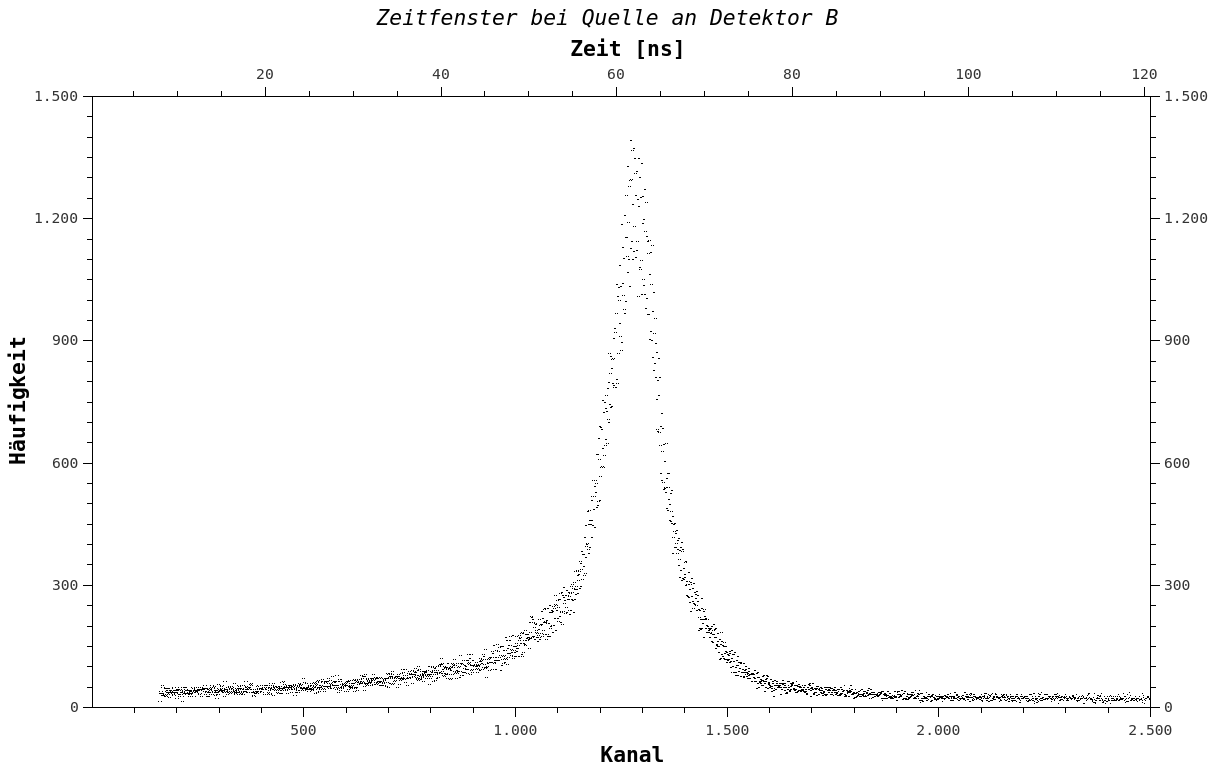
\includegraphics[width=1.2\textwidth, height=0.225\textheight]{pic/T_B_dia.png}
                \label{dfd:T_B}
            \minipend \\
            \minipanf
                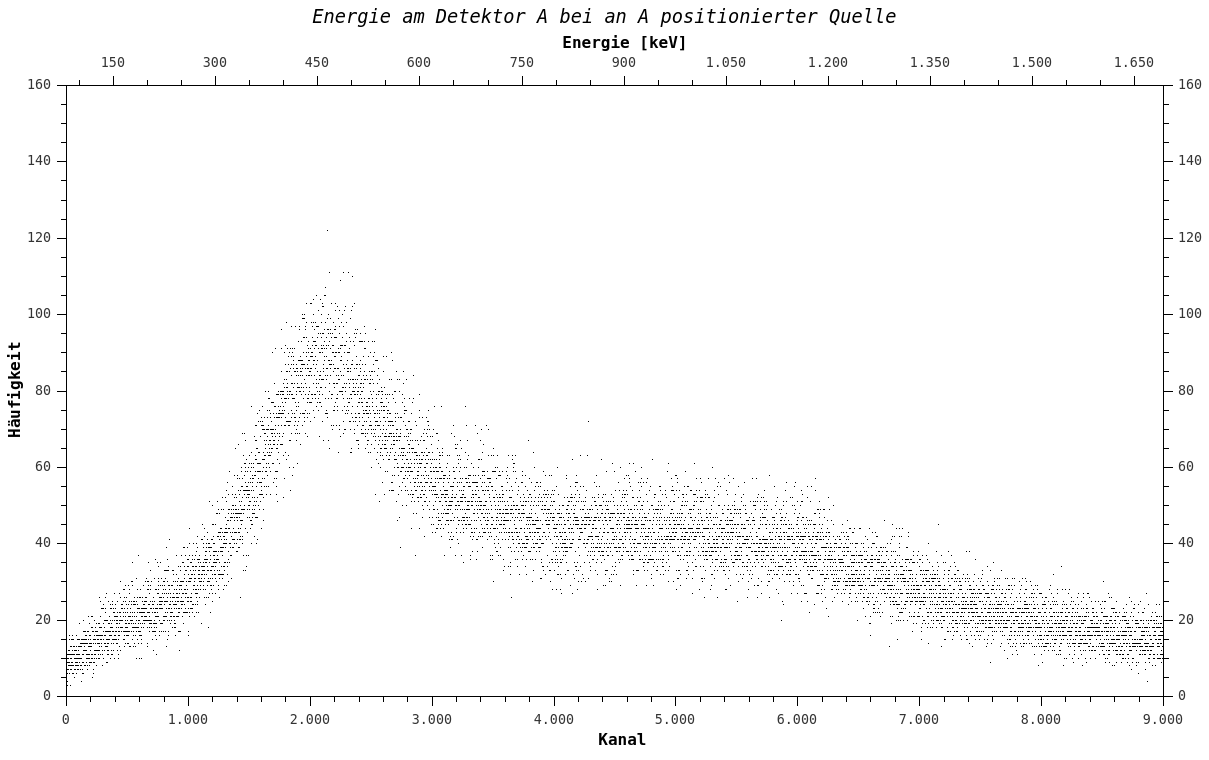
\includegraphics[width=1.2\textwidth, height=0.225\textheight]{pic/Efenster_DetA_A.png}
                \label{dfd:EdetAA}
            \minipend
            &
            \hspace{9mm} 
            \minipanf 
                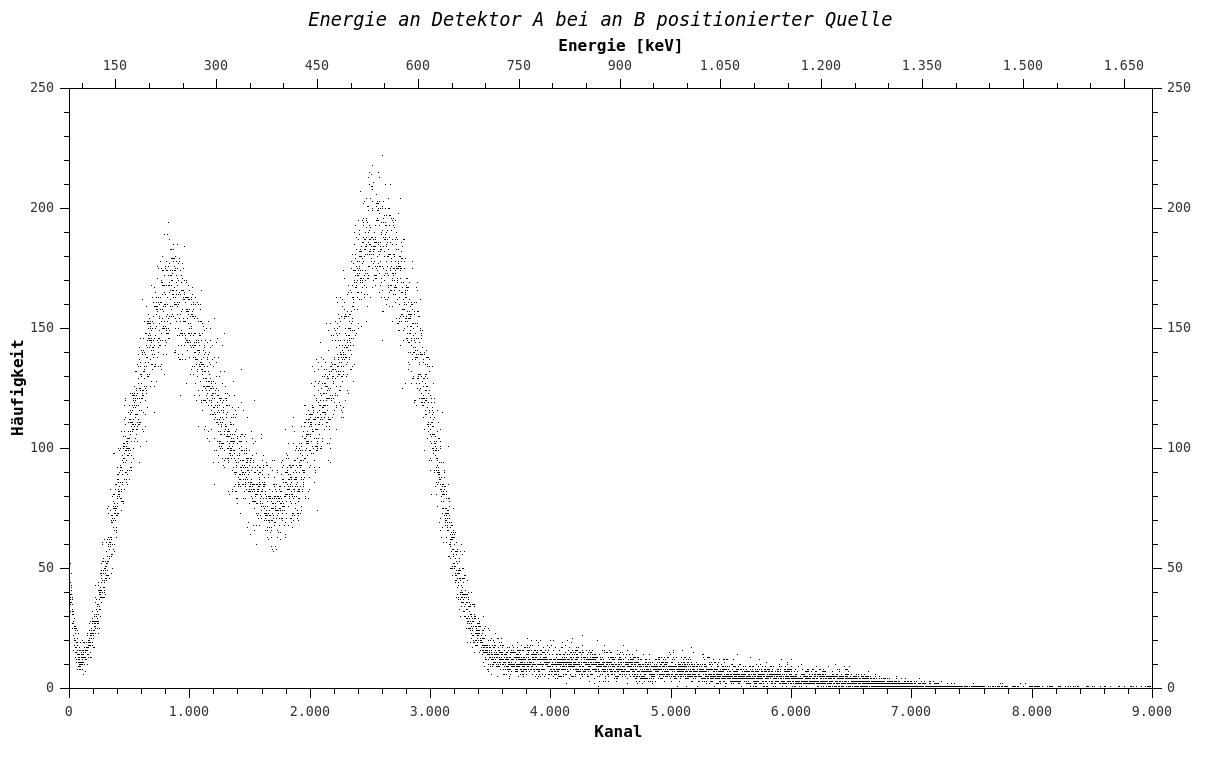
\includegraphics[width=1.2\textwidth, height=0.225\textheight]{pic/Efenster_DetA_B.png}
                \label{dfd:EdetBA}
            \minipend \\
            \minipanf 
                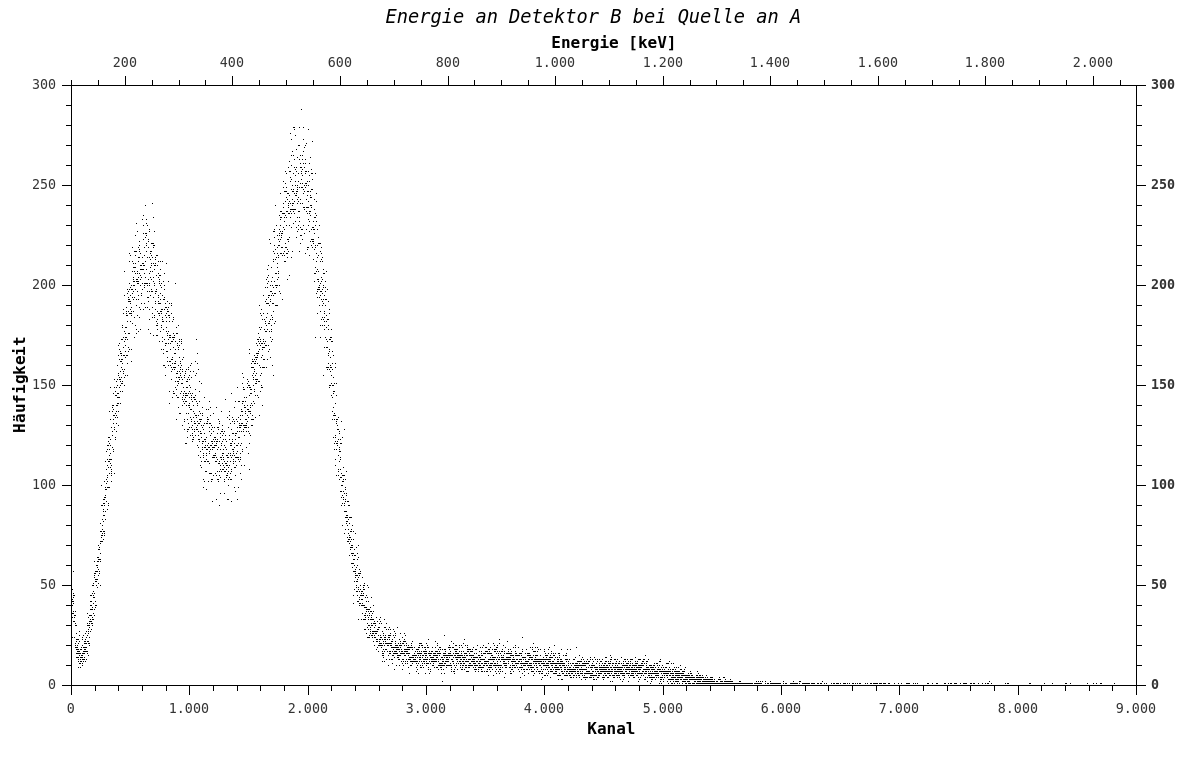
\includegraphics[width=1.2\textwidth, height=0.225\textheight]{pic/Efenster_DetB_A.png}
                \label{dfd:EdetAB}
            \minipend
            &
            \minipanf 
                \hspace{9mm}
                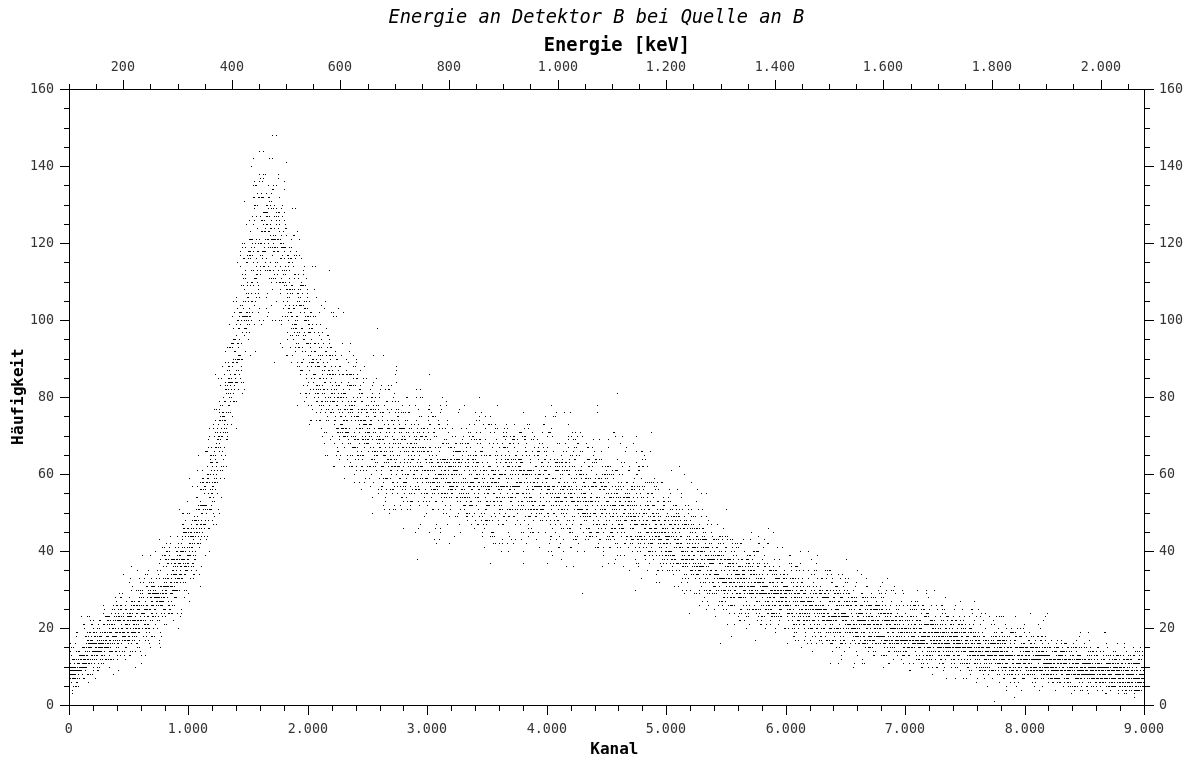
\includegraphics[width=1.2\textwidth, height=0.225\textheight]{pic/Efenster_DetB_B.png}
                \label{dfd:EdetBB}
            \minipend \\            
        \end{longtable}
        \captionof{figure}{Gegenüberstellung der Messungen mit der Quelle an Det. A (links) und Det. B (rechts)}
        \label{dft:kaliAB}
    Aus den Zeitdiagrammen, die auf den ersten Blick sehr ähnlich sind, kann man über einen Gauß-Fit die Peak-Positionen, das heißt, die Maxima, bestimmen.
    Diese wird verwendet, um die Laufzeitdifferenz und damit letztlich den Abstand zwischen den Detektoren A und B zu bestimmen.
    Die Zeitpeaks liegen bei $ \Delta t_A = \unit[63,35]{ns}$ und $\Delta t_B = \unit[61,80]{ns}$. Um nun den Detektorabstand zu bestimmen müssen wir berücksichtigen, dass ein hardwareseitiges Delay $t_{HW}$ die Koinzidenzzeitmessungen beeinflusst. Dieses Delay würden wir mit zwei Photonen, die sich direkt vor den Detektoroberflächen befinden, ermitteln können, d.h. der Peak der Zeitmessung wäre bei $t_{HW}$. Verschieben wir nun die Quelle vor Detektor A, so ist dieser Peak um die Laufzeit des einen Photons zu Detektor B verschoben, d.h. $t_A = t_{HW} - D/c$. Analog ergibt sich für die Messung vor Detektor B der Peak bei $t_B=t_{HW} + D/c$. Durch Differenzbildung der Peakmitten eliminieren wir die Abhängigkeit von der Delayzeit: $\Delta T = t_B - t_A = 2D/c $. Somit erhalten wir für den Detektorabstand:
    \begin{equation*}
    	l = \frac{1}{2}\cdot c \cdot \Delta T = 23,25\ \unit{cm}
    \end{equation*}
    Dieser Wert ist kleiner als der in der Anleitung angegebene. Diese Art von Messung ist vermutlich nicht exakt genug, um den Detektorabstand hinreichend genau zu bestimmen.

        
    \subsubsection{Schwerpunktsdiagramme}
    Als nächstes sind die Schwerpunktsdiagramme zu betrachen. Es wurden drei von Detektor A erstellt. Einmal als die Quelle an Detektor B positioniert wurde, danach an Detektor A und einmal mittig zwischen beiden.\\
    In Abbildung \ref{dfp:SPDdetB} kann gegenüber \ref{dfp:SPDMitte} ein schwächeres Muster erkannt werden. Gegenüber Abbildung \ref{dfp:SPDMitte} ist in beiden deutlich die Kristallstruktur erkennbar.
    Diese stellt sich durch die vielen Maximumflecken dar. Gekennzeichnet werden die Kristalle durch ein rotes Gitter, welches vom PC über die Bilder gelegt wurde. Dieses kennzeichnet die 8x8-Matrix.\\
        
    \begin{tabular}{p{5cm}p{5cm}p{5cm}c}
        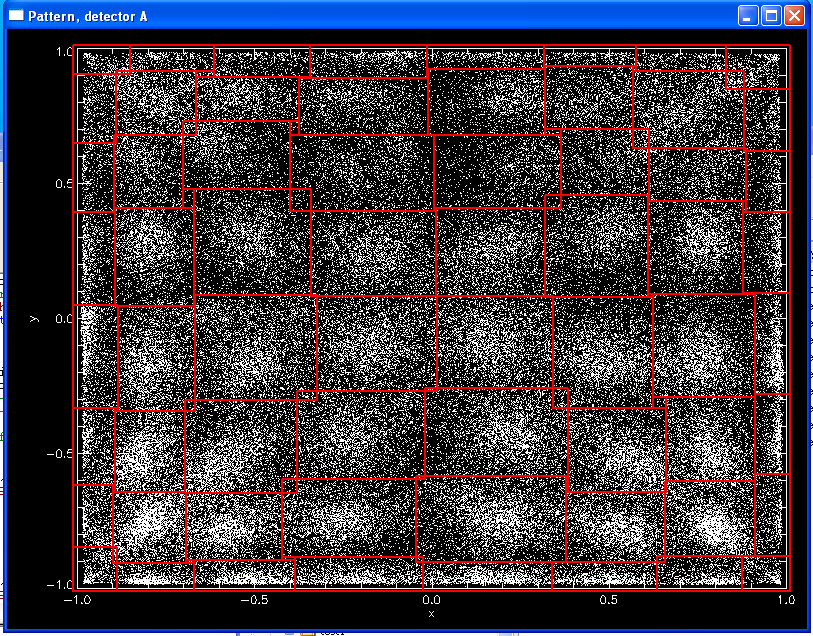
\includegraphics[width=0.3\textwidth, height=0.2\textheight]{pic/Einzelfenster_Bilder/fenster_DetAanB.png}
        \captionof{figure}{Messung bei Quelle an Detektor B}
        \label{dfp:SPDdetB}
        &
        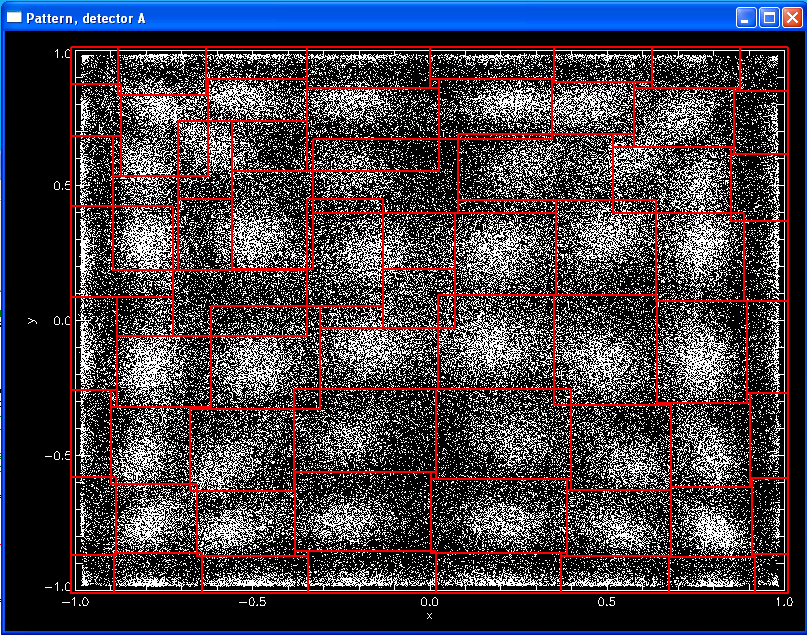
\includegraphics[width=0.3\textwidth, height=0.2\textheight]{pic/Einzelfenster_Bilder/fenster_DetAMitte.png}
        \captionof{figure}{Messung bei Quelle in der Mitte}
        \label{dfp:SPDdetA}
        &
        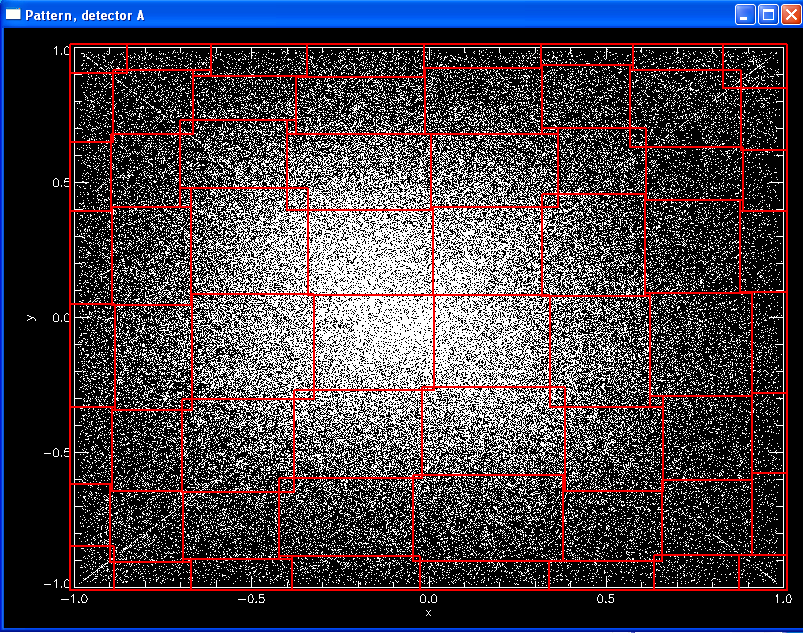
\includegraphics[width=0.3\textwidth, height=0.2\textheight]{pic/Einzelfenster_Bilder/fenster_DetAanA.png}
        \captionof{figure}{Messung bei Quelle an Detektor A}
        \label{dfp:SPDMitte}
    \end{tabular}\\
    
    Bei der Messung an Quelle A zeigt sich auch deutlich, wie die Kristalle geschnitten wurden. So finden hier an den Einschnitten keine Reflexionen statt und die Strahlung kann sich kugelförmig ausbreiten und als großer
    kreisförmiger Hotspot detektiert werden. Es können allerdings auch vier Dreiecke beobachtet werden, welche durch die Kristallstruktur erzeugt wurden.
    Im Bild der Messung des Detektors A während sich die Quelle an Detektor B befand ist weiterhin erkennbar, dass widererwartend die Intensität in der oberen Bildhälfte schwächer ist als in der unteren. Die Schwächung
    sollte normalerweise in der unteren Hälfte auftreten, da hier eine Glasplatte Strahlung abschirmt. Das heißt, das Bild muss um 180° gedreht sein. 
    Sehr schön sind in den Abbildungen \ref{dfp:SPDdetB} und \ref{dfp:SPDMitte} auch die Verzerrungen sichtbar, die durch die Projektion der kugelförmigen Ausbreitung der Strahlung auf eine ungekrümmte Ebene entstehen.
        
    \subsection{Tomografische Messungen}
    Im Folgenden wird die eigentlich Datenerfassung und Auswertung beschrieben.
    	\subsubsection{Messung einer Quellkonfiguration, Phantom isotroper Dichteverteilung}
    	        \textbf{Hauptversuch}\\
    	        
    	        Als nächsten wurde eine Messung mit unbekannter Quellverteilung gestartet. Die Energie- und das Zeitfenster entsprechen den oben bestimmten Intervallen. Der Detektor fährt dann unter gewissen Winkeln $\theta$ die $30\ \unit{BIN} = 101,25\ \unit{mm}$ breite s-Achse mit einer Geschwingigkeit von $22\ \unit{mm/s}$ ab. Dabei wird für gewisse Positionen die Anzahl der Konzidenzereignisse in Abhängigkeit der s-Koordinate aufgenommen. Dies wird für alle Winkel im Abstand von $2\unit{°}$ Schritten wiederholt, wodurch das Sinogramm entsteht, welches in folgender Abbildung dargestellt wird:\\ 
    				
    			\begin{tabular}{p{6cm}p{6cm}}
    				  \minipanf 
    				      	\begin{center}
    				      	
    				      		\makebox[\linewidth]{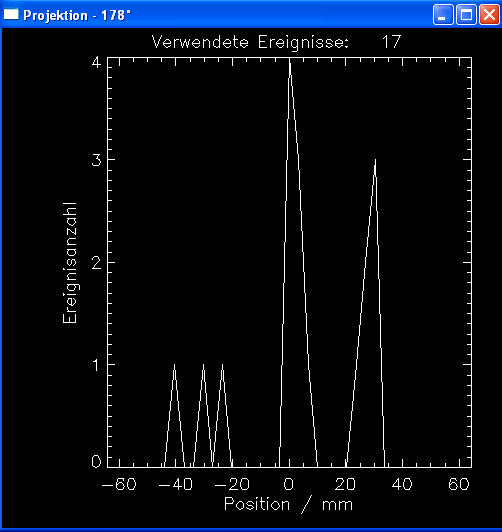
\includegraphics[width=1.\textwidth, height=0.2\textheight]{pic/Einzelfenster_Bilder/unbekannte_Quelle/unbek_festerWinkel.png}}  
    				      		\caption*{\footnotesize{Koinzidenzereigniszahl zu festem Winkel}}   
    				      	
    				      	\end{center}             
    				   \minipend
    				   &
    				   \hspace{10mm} 
    				   \minipanf
    				   		\begin{center}
    				       		 	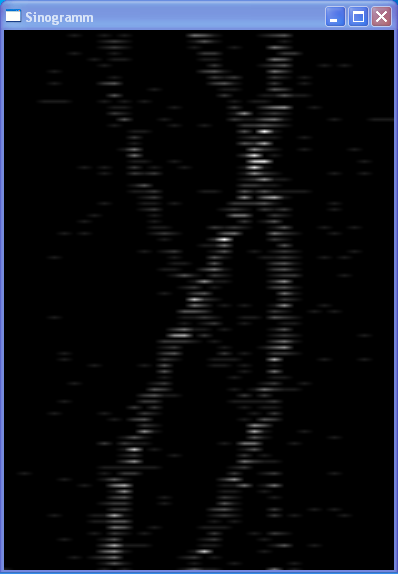
\includegraphics[width=1.\textwidth, height=0.2\textheight]{pic/Einzelfenster_Bilder/unbekannte_Quelle/unbek_sino.png}
    				        		\caption*{\footnotesize{Sinogramm - horizontal: s; vertikal: $\theta$;\\ Helligkeit: Ereigniszahl}} 
    				        \end{center}
    				   \minipend \\              
    			\end{tabular}\\
    			\ \\
    			Dabei entspricht jeder Graph der linken Art einer in Graustufen dargestellte Linie im Sinogramm. Die so erhaltenen Daten können nun genutzt werden, um eine inverse Radon-Transformation auf sie anzuwenden, um die ursprüngliche Quellverteilung zu erhalten. Aus jeder 'Zeile' des Sinogramms können wir nun analog zum Vorgehen im Abschnitt (\ref{dfd:Radon}) eine rückprojizierte Matrix extrahieren, die man zur Gesamtrückprojektion aufsummiert. Je mehr Winkel der Detektor abfährt, desto mehr Summanden enthält die Rückprojektion und desto klarer wird das Bild. Bevor man die inverse Transformation durchführt, kann noch ein Filter auf das Sinogramm angewendet werden. Im konkreten Experiment lag eine Verteilung, die aus drei Punktquellen bestand, vor, welche in der folgenden Bilderserie schrittweise rekonstruiert wurde. Weiterhin wurde ein Ramp-Filter mit Dimension $d=13$ verwendet, um einen direkten Vergleich zu haben:\\
    	        \begin{longtable}{p{7cm}p{7cm}c}
    	                \textbf{ungefilterter Projektion} & \textbf{gefilterte Rückprpjektion} \endhead
    	                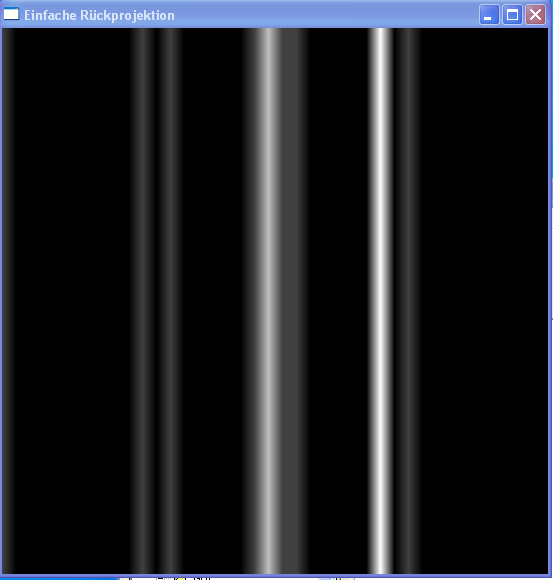
\includegraphics[width=0.3\textwidth, height=0.2\textheight]{pic/Einzelfenster_Bilder/unbekannte_Quelle/unbek1_einf_prj.png}
    	                & 
    	                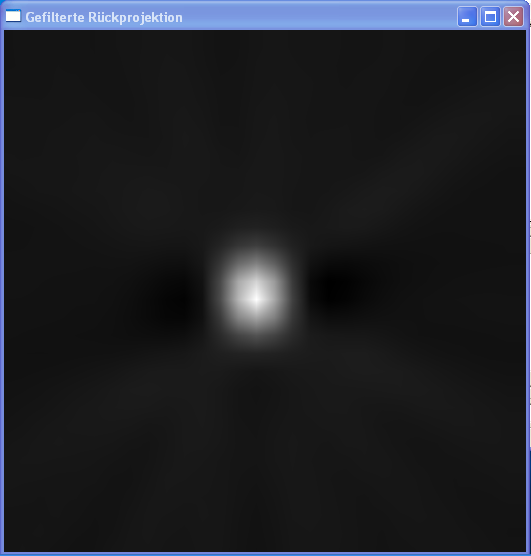
\includegraphics[width=.3\textwidth, height=0.2\textheight]{pic/Einzelfenster_Bilder/unbekannte_Quelle/unbek1gef_prj.png}\\
    	                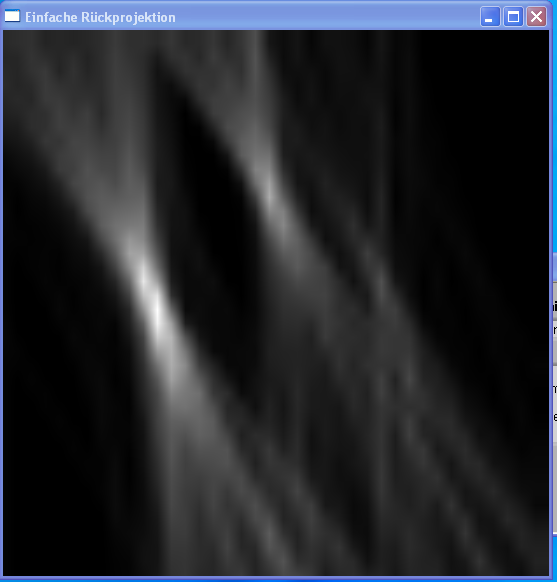
\includegraphics[width=0.3\textwidth, height=0.2\textheight]{pic/Einzelfenster_Bilder/unbekannte_Quelle/unbek2einf_prj.png}
    	                & 
    	                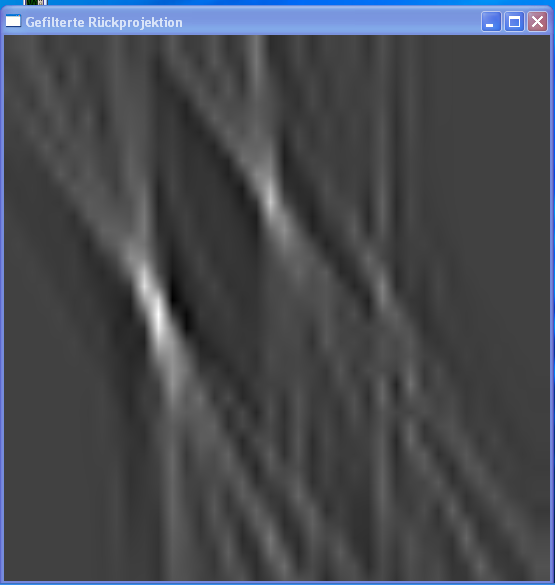
\includegraphics[width=.3\textwidth, height=0.2\textheight]{pic/Einzelfenster_Bilder/unbekannte_Quelle/unbek2gef_prj.png}\\ 
    	                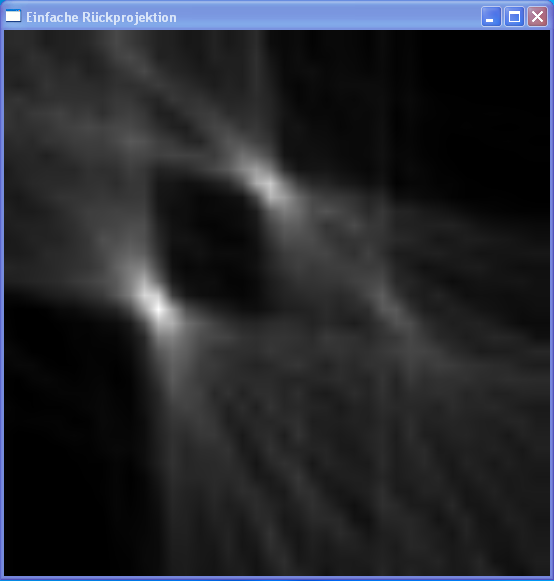
\includegraphics[width=0.3\textwidth, height=0.2\textheight]{pic/Einzelfenster_Bilder/unbekannte_Quelle/unbek3einf_prj.png}
    	                & 
    	                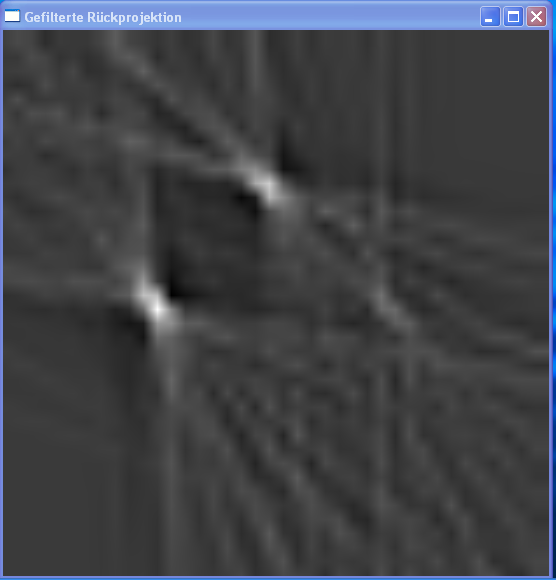
\includegraphics[width=.3\textwidth, height=0.2\textheight]{pic/Einzelfenster_Bilder/unbekannte_Quelle/unbek3gef_prj.png}\\               
    	                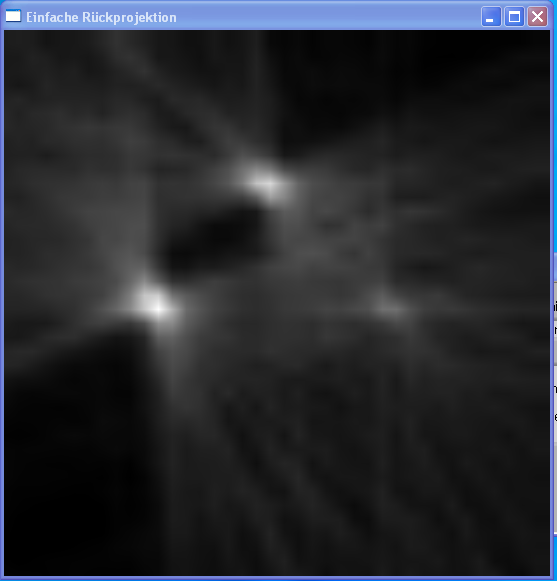
\includegraphics[width=0.3\textwidth, height=0.2\textheight]{pic/Einzelfenster_Bilder/unbekannte_Quelle/unbek4einf_prj.png}
    	                & 
    	                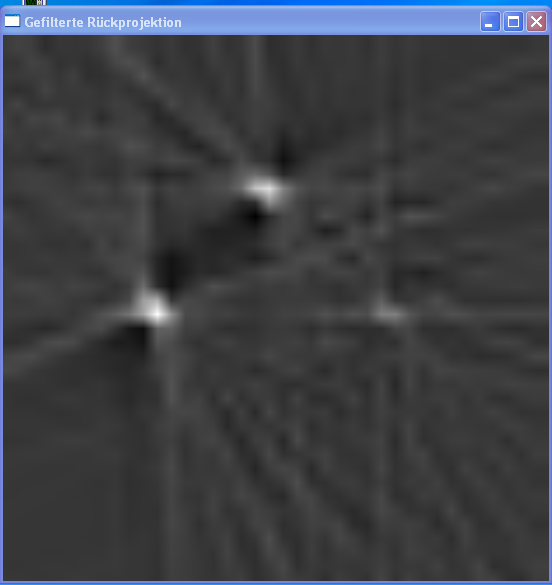
\includegraphics[width=.3\textwidth, height=0.2\textheight]{pic/Einzelfenster_Bilder/unbekannte_Quelle/unbek4gef_prj.png} \\
    	            \end{longtable}
    	            \captionof{figure}{Screenshots der Bildenstehung der gefilterten (rechts) und ungefilterten (links) Rückprojektion}
    	            \ \\
    	            
    	            \textbf{Untersuchung des Einflusses verschiedener Filter}\\
    	            
    	            Wie man in der zuvorgehenden Rekonstruktion bereits gesehen hat, haben Filter einen Einfluss auf den Kontrast und die Genauigkeit der Ortsbestimmung der hellen Peaks in der Rückprojektion. Deshalb wurde in einer Offline-Nachbearbeitung die Anwendung verschiedenster Filter getestet:
    	            \begin{center}
    	              \begin{longtable}{p{4.0cm}p{4.0cm}p{4.0cm}l}
    	                  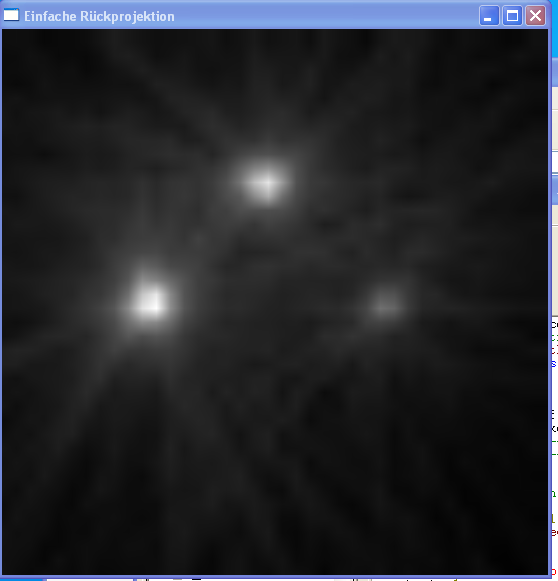
\includegraphics[width=0.25\textwidth, height=0.15\textheight]{pic/Einzelfenster_Bilder/unbekannte_Quelle/unbek5_einf_prj.png}
    	                  ungefilterte Rückprojektion
    	                  & 
    	                  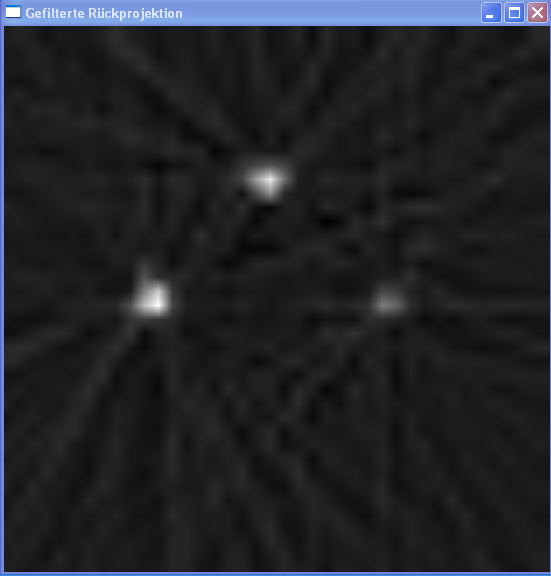
\includegraphics[width=.25\textwidth, height=0.15\textheight]{pic/Einzelfenster_Bilder/unbekannte_Quelle/unbek5_ramp.png}
    	                  Ramp-Filter
    	                  &
    	                  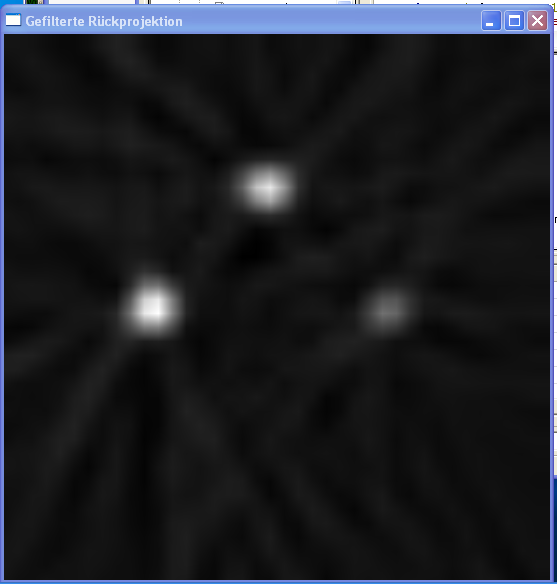
\includegraphics[width=0.25\textwidth, height=0.15\textheight]{pic/Einzelfenster_Bilder/unbekannte_Quelle/unbek5_hanning_weighted.png}
    	                  Hanning-weighted-Filter\\
    	                  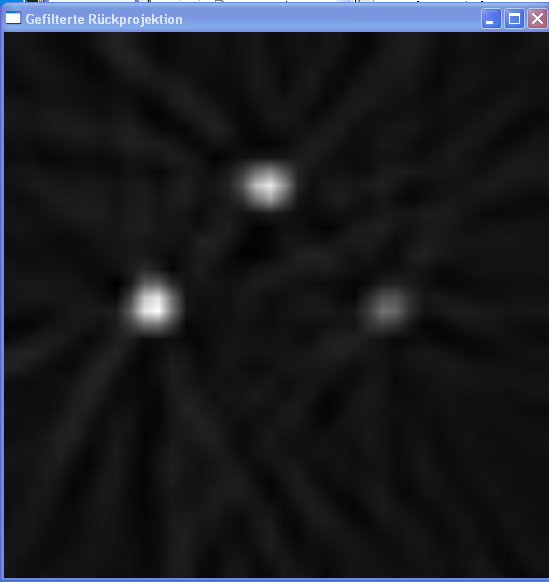
\includegraphics[width=.25\textwidth, height=0.15\textheight]{pic/Einzelfenster_Bilder/unbekannte_Quelle/unbek5_middle.png} 
    	                  Middle-Filter
    	                  &
    	                  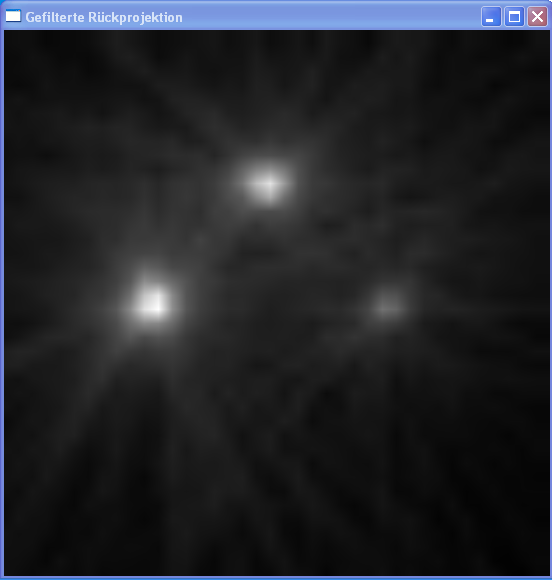
\includegraphics[width=0.25\textwidth, height=0.15\textheight]{pic/Einzelfenster_Bilder/unbekannte_Quelle/unbek5_rausch3.png}
    	                  Rauschfilter bei Dimension 3
    	                  & 
    	                  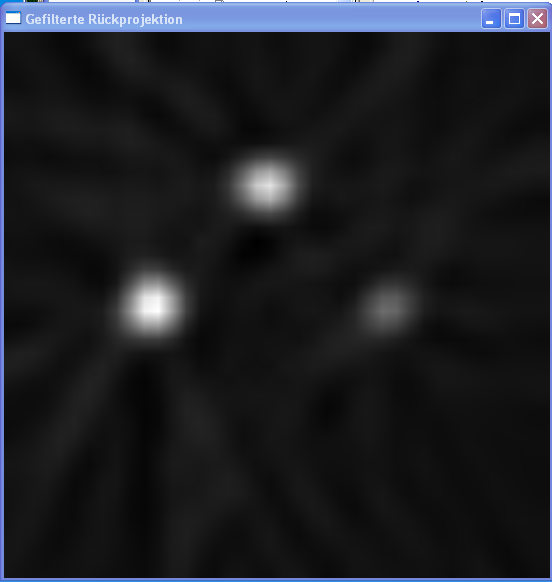
\includegraphics[width=.25\textwidth, height=0.15\textheight]{pic/Einzelfenster_Bilder/unbekannte_Quelle/unbek5_rausch13.png}               
    	                  Rauschfilter bei Dimension 13\\
    	                  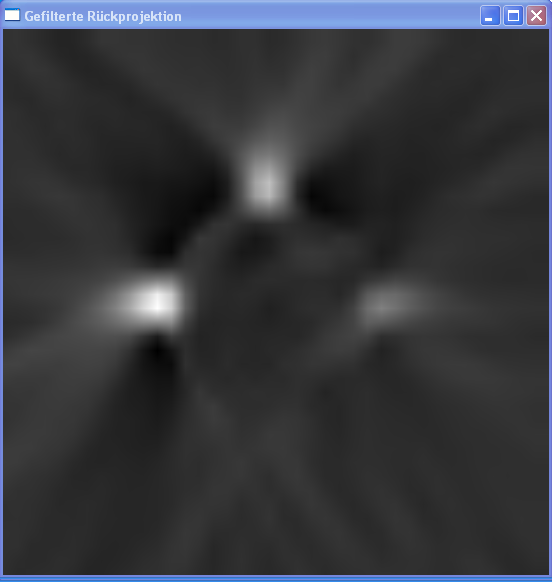
\includegraphics[width=0.25\textwidth, height=0.15\textheight]{pic/Einzelfenster_Bilder/unbekannte_Quelle/unbek5_rausch25.png}
    	                  Rauschfilter bei Dimension 25
    	                  &
    	                  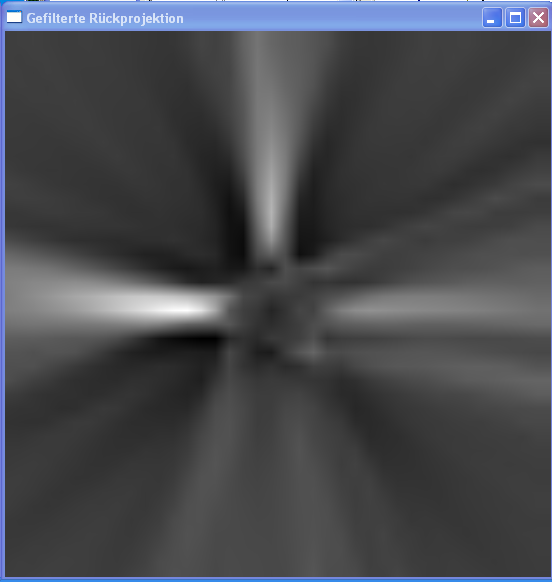
\includegraphics[width=.25\textwidth, height=0.15\textheight]{pic/Einzelfenster_Bilder/unbekannte_Quelle/unbek5_rausch36.png} 
    	                  Rauschfilter bei Dimension 36
    	                  &
    	                  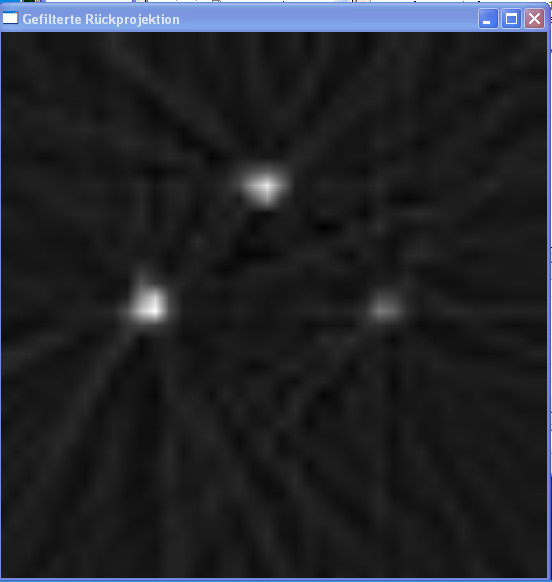
\includegraphics[width=.25\textwidth, height=0.15\textheight]{pic/Einzelfenster_Bilder/unbekannte_Quelle/unbek5_shepp-logan.png}
    	                  Shepp-Logan-Filter
    	                \end{longtable}
    	            \end{center}
    	            \vspace{5mm}
    	            Der Hanning-Weighted-, der Middle- und der Rauschfilter heben allesamt die strahlförmigen Strukturen, die von den Quellen ausgehen hervor und lassen die Quellen selbst etwas 'verwaschener' wirken. Dadurch heben sie sich zwar besser vom Untergrund ab, lassen sich allerdings schwerer lokalisieren. Außerdem bilden sich dunkle Bereiche um die Peaks. Dadurch könnte ihre Anwendung in der Praxis dann von Bedeutung sein, wenn es darum geht, kompliziertere Quellverteilungen zu analysieren, bei denen eine exakte Lokalisierung der Peaks nicht vordergründig ist. Weiterhin wurde der Einfluss der Dimension beim Rauschfilter untersucht: Je größer diese wurde, desto verwaschener wurde das Bild bis zur vollkommenen Unkenntlichkeit.\\
    	            
    	            Ganz im Gegensatz zum Ramp-Filter und dem Shepp-Logan-Filter: Sie erzeugen beide ein recht scharfes Bild der Peaks. Um dies besser zu analysieren betrachten wir die Messwerte des Ramp-Filters verglichen mit der ungefilterten Variante in einer 3D-Darstellung:\\
    	            
           \minipanf
           \begin{tabular}{p{6cm}p{6cm}c}
                            \minipanf 
                                \makebox[\linewidth]{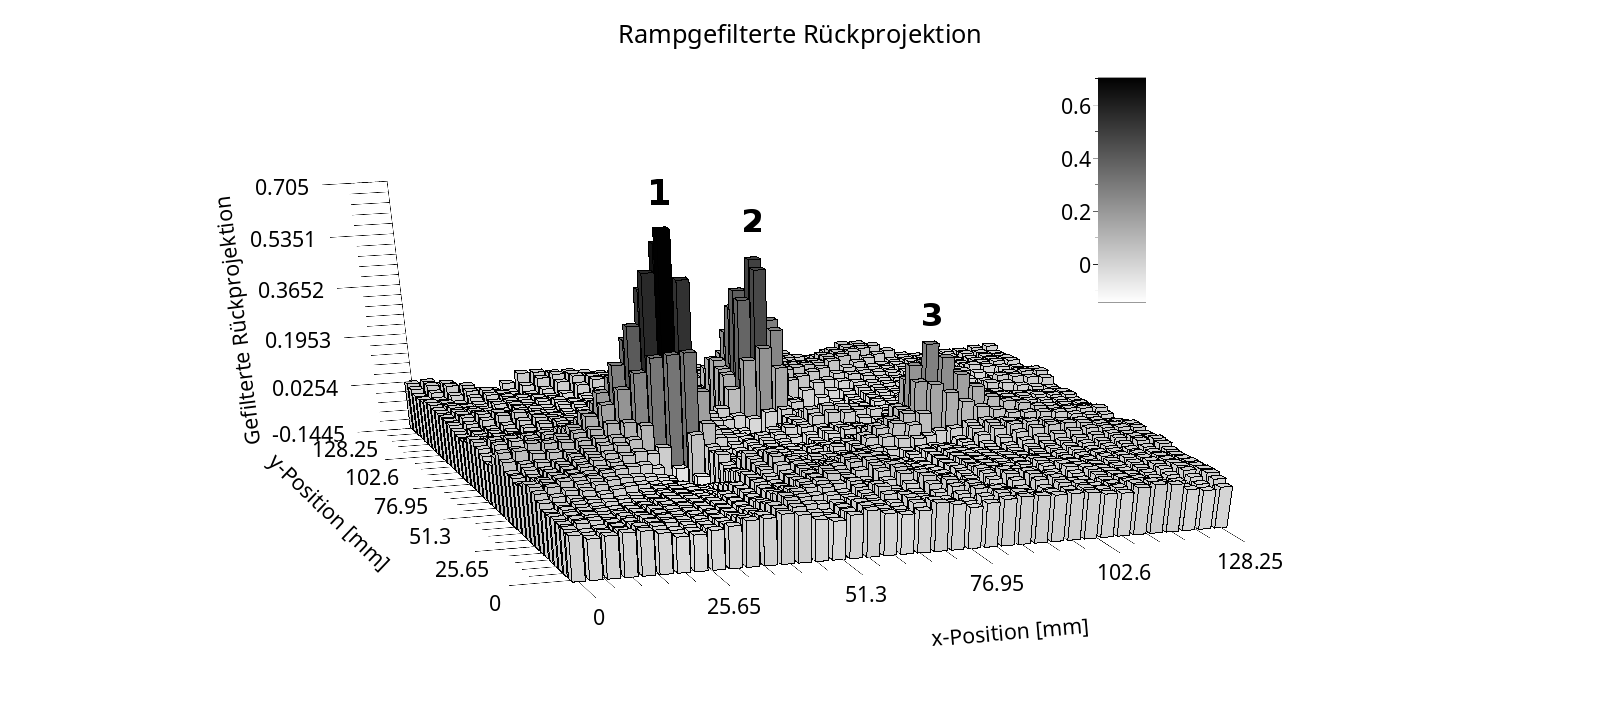
\includegraphics[width=1.5\textwidth, height=0.3\textheight]{pic/3dPlotTomographRamp.png}} 
                            \minipend
                            &
                            \hspace{5mm} 
                            \minipanf
                                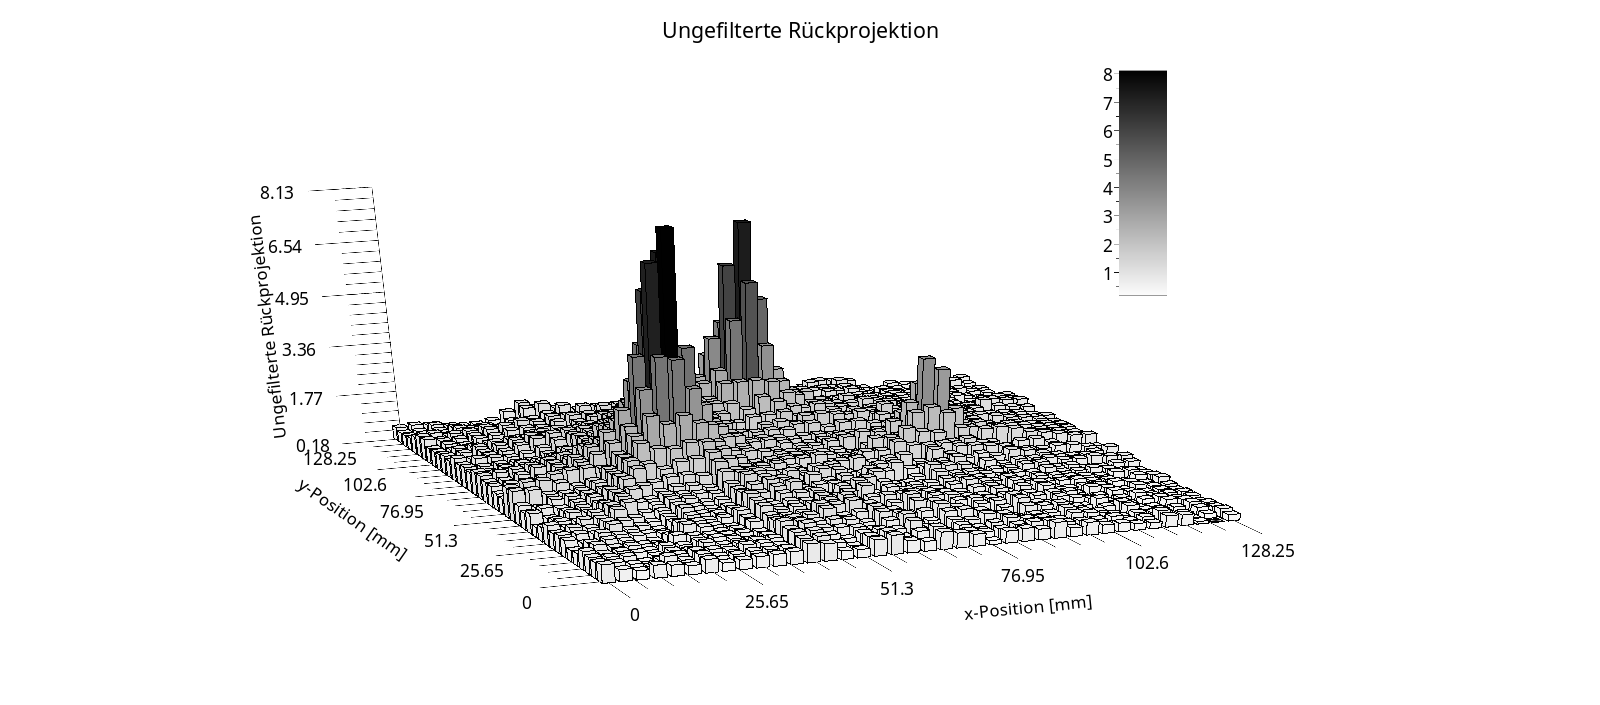
\includegraphics[width=1.5\textwidth, height=0.3\textheight]{pic/3dPlotTomographUngef.png}
                            \minipend \\              
             \end{tabular} 
            \captionof{figure}{Gefilterte und Ungefilterte Rückprojektion der Aktivitätsverteilung}
            \label{dfd:AKV}
            \minipend
            \ \\
            
            Der verwendete Rampfilter kann, wie im Abschnitt (\ref{dfd:Radon}) bereits ausführlich aufgeführt, als eine Faltung des Sinogramms $p(s,\theta)$ mit einer Filterfunktion $h(s)$ zu einem festen Winkel $\theta$ dargestellt werden. Das heißt man addiert zu einem festen Wert von $p(s,\theta)$ die umliegenden Funktionswerte innerhalb eines Bereiches von $d$ = 13 BINs mit einem (negativen) Gewicht. Man beobachtet, dass durch diese Faltung im Vergleich zur ungefilterten Rückprojektion ein höheres Untergrundrauschen in Bereichen mit geringer Aktivität entsteht, da insbesondere auch die Skala einen kleineren Bereich ($N_{ramp}(x,y) \in [-0,14,\ 0,7],\ N_{u}(x,y) \in [0,18,\ 8,13] $) abdeckt. Allerdings fallen die Peaks deutlich schneller ab (negative Bereiche um Maximum), wodurch man sie besser lokalisieren kann. Aus diesem Grund wird im Folgenden der gefilterte Datensatz für die quantitative Auswertung verwendet.\\
            
            \textbf{Quantitative Auswertung}\\
            
            \begin{tabular}{p{12cm}	p{0.5\textwidth}}            	
            	\minipanf
            		Zunächst werden die Positionen $(x_i,y_i) (i = 1,2,3)$ der 3 Quellen im verschlossenen Plastikbehältnis bestimmt. Dafür wird die in Abbildung (\ref{dfd:AKV}) visualisierte Rückprojektion $N(x,y)$ verwendet, die durch Auslesen der in \texttt{Matrix\_reco.txt} enthaltenen Messwertmatrix entstanden ist. Der erste Eintrag sei als Koordinatenursprung gewählt. 1 BIN des Rekonstruktionsrasters entspricht $3,375\ \unit{mm}$. Die Positionen der Quellen werden mit den lokalen Maxima $N(x_i,y_i)$ der Aktivitätsverteilung identifiziert.\\
            		Anschließend quantifiziert man die Aktivität jeder einzelnen Quelle, indem man die rückprojizierten Verteilung über einen kleinen Bereich um die Peaks mittelt. Bezeichne diesen Mittelwert mit $\bar{N}(x_i,y_i)$. Im Rahmen dieser Auswertung wurde ein quadratischer Bereich gewählt, in welchem Werte anzutreffen waren, die in der Nähe des FWHM (=Full Width Half Maximum) lagen. Dieses Vorgehen wird durch die nebenstehende Abbildung visualisiert.
            	\minipend            
            	&
            	\begin{minipage}[c]{\textwidth}
                	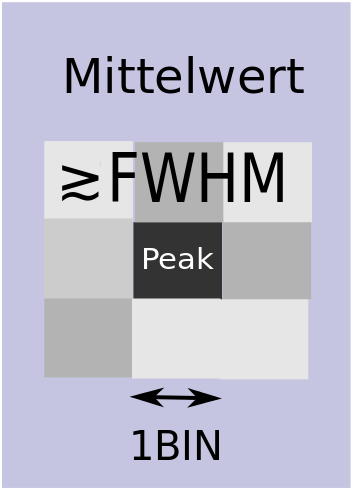
\includegraphics[width=0.25\textwidth, height=0.20\textheight]{pic/Skizze_Mittelung.png}
                \end{minipage}
            \end{tabular}\\
            
            Mittels einfacher Verhältnisbildung können unter Vorgabe einer Referenzaktivität $A_{ref}$ nun unbekannte Aktivitäten innerhalb der Verteilung berechnet werden. Dabei wurde die stärkste Aktivität mit $A_0 \equiv A(t_0 = \textrm{01.02.2010}) = (363 \pm 11)\ \unit{kBq}$ angegeben. Mit dem Aktivitätsgesetz kann man nun berechnen:
            
            \begin{equation}
            	A_{ref} \equiv A(t =\textrm{29.10.2015}) = A_0 \cdot \left( \frac{1}{2}\right)^{\frac{t-t_0}{T_{1/2}}} = (79 \pm 3)\ \unit{kBq}
            \end{equation}\\
            Wobei die Halbwertszeit $T_{1/2}(^{22}\textrm{Na}) = (2,6027 \pm 0,0010)\ \unit{a}$ verwendet wurde, sowie folgende Fehlerformel:
            \begin{equation}
                \left(\frac{\Delta A_{ref}}{A_{ref}}\right)^2 = \left(\frac{\Delta A_0}{A_0}\right)^2 + \left(\ln(2) \cdot \frac{\Delta T_{1/2}}{T_{1/2}}\right)^2
            \end{equation}\\   
            Bezeichnet man $A_{ref} \propto \bar{N}_{ref} \equiv \bar{N}(x_1,y_1)$ als rückprojizierte Aktivität der Referenzquelle, so erhält man für die unbekannten Aktivitäten $A_i \propto \bar{N}(x_i,y_i)$:
            \begin{equation}
            	A_i = A_{ref} \cdot \frac{\bar{N}(x_i,y_i)}{\bar{N}_{ref}}
            \end{equation}    
            \begin{equation}
                 \left(\frac{\Delta A_i}{A_i}\right)^2 = \left(\frac{\Delta A_{ref}}{A_{ref}}\right)^2 + \left(\frac{\Delta \bar{N}(x_i,y_i)}{\bar{N}(x_i,y_i)}\right)^2 + \left(\frac{\Delta \bar{N}_{ref}}{\bar{N}_{ref}}\right)^2
             \end{equation}\\   
             Hierbei wurden die Fehler der rückprojizierten Aktivitäten als Standardabweichungen des Mittelwertes gesetzt, die sich beim obigen Mittelvorgang ergab: $\Delta \bar{N}(x_i,y_i) = \sigma(\bar{N})$. Die systematischen Fehler des PET-Scanners waren leider nicht bekannt. Zusammenfassend ergeben sich folgende Resultate:\\
             
             \begin{tabular}{c|c|c|c|c|c}
             				Peak \# $i$ 	& 	$x_i$ [mm] 	& 	$y_i$ [mm] 	& Peakmaximum $N(x_i, y_i)$ & Peakmittel $\bar{N}(x_i,y_i)$ & $A_i$ [kBq]\\
             	\hline		$1$				&	$37 \pm 3,4$& $64 \pm 3,4$&	$0,705$					& $0,50 \pm 0,05$				& $79 \pm 2,4$\\
             				$2$				&	$64 \pm 3,4$& $94 \pm 3,4$&	$0,4933$				& $0,36 \pm 0,03$				& $57 \pm 7,4$\\
             				$3$				&	$91 \pm 3,4$& $64 \pm 3,4$&	$0,2837$				& $0.20 \pm 0,02$				& $31 \pm 4,1$\\
             \end{tabular}
             \caption{Aktivitäts- und Positionsbestimmung der unbekannten Quellverteilung}
             \vspace{3mm}  
                      
             Da die Peaks eine gewisse Breite haben, die sich in der gefilterten Darstellung über etwa drei BINs erstreckt, wurde ein Ortsfehler von einem BIN angenommen. Diese Ortsunbestimmtheit in Verbindung mit den diskreten Messwerten führt zu einer Begrenzung der Ortsauflösung. Das heißt, dass es einen minimalen Abstand $d_{min}$ zwischen zwei Peaks gibt, unterhalb dessen man sie nicht mehr unterscheiden kann. In der Optik bestimmt man Auflösungen mit Hilfe des heuristischen \textit{Rayleigh-Kriteriums}, das besagt, dass der Mindestabstand zweier Lichtquellen gleich dem Abstand des Minimums erster Ordnung vom Zentrum des Beugungsmusters ist. Dieses Kriterium ist hier nicht anwendbar, da wir nicht zwangsläufig klar identifiziertbare Minima haben. Aus diesem Grund wurde die oben erläuterte Variante mit der Halbwertsbreite hier erneut angewendet: Der minimale Abstand zwischen zwei (identischen) Maxima entspricht der doppelten Distanz der Peakmitte zur Position der Halbwertsbreite. Folgende Abbildung verdeutlicht dies:\\
             
             \begin{tabular}{p{4.5cm}p{4.5cm}p{4.5cm}c}
                                          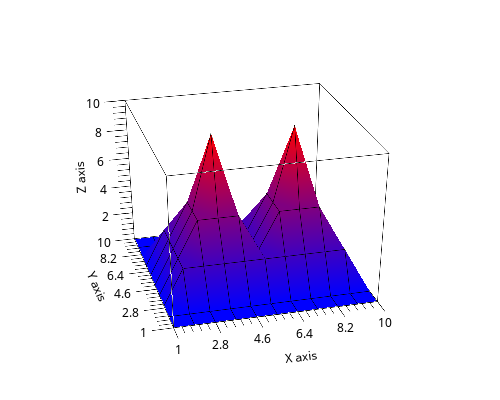
\includegraphics[width=0.375\textwidth, height=0.2\textheight]{pic/3dplotAufloes3.png}
                                         & 
                                          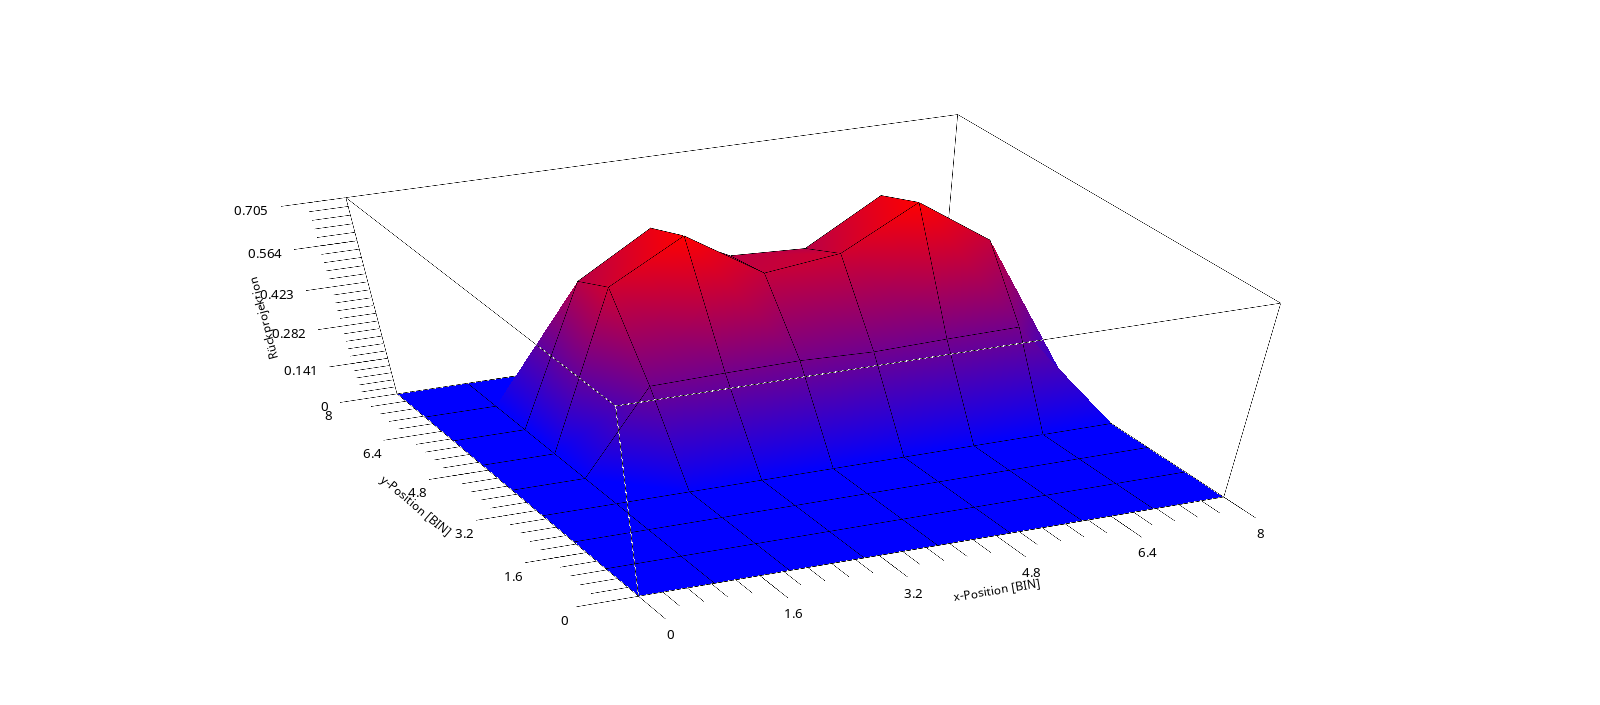
\includegraphics[width=0.375\textwidth, height=0.2\textheight]{pic/3dplotAufloes2.png}
                                         &
                                          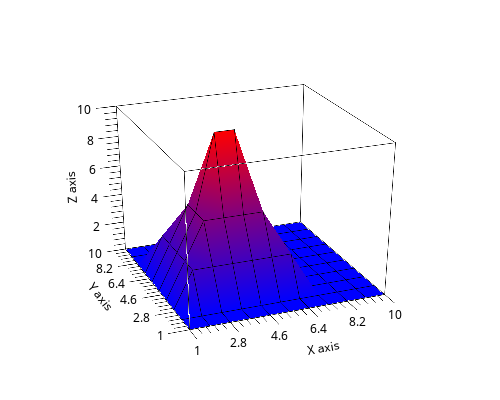
\includegraphics[width=0.375\textwidth, height=0.2\textheight]{pic/3dplotAufloes1.png} \\               
                          
             \end{tabular}
             \captionof{figure}{Kriterium zur Unterscheidung zweier Peaks}
             \label{dfd:Auflösung}
             \vspace{3mm}
             
             In der ungefilterten Darstellung war die Halbwertsbreite bereits innerhalb von einem BIN erreicht, wodurch sich eine Ortsauflösung von ungefähr $d_{min} = 2\ \unit{BIN} = 6,75\ \unit{mm}$ ergibt.
            
              
                   
        \subsubsection{Messung mit einer Punktquelle, Phantom an-/isotroper Dichteverteilung}
        
        \textbf{Qualitative Gegenüberstellung an-/isotroper Dichteverteilung}\\
        Nun sollen eine isotrope und eine anisotrope Dichteverteilung des Quellbehältnisses untersucht werden. In der nachstehenden Tabelle ist die Entwicklung der Rückprojektionen
        protokolliert. Man kann hier früh erkennen, dass die gefilterten Bilder die Quelle schärfer abbilden als die ungefilterten. Besonders sind allerdings die Screenshots 
        der abgeschlossenen Messung und  die fertigen Sinogramme. Bei der isotropen Messung kann man klar die isotrope erkennen. Die Intensität im Sinogramm ist kontinuierlich gleich,
        ebenso ist in der gefilterten Rückprojektion kein Schatten mehr erkennbar. 
 
              \begin{longtable}{p{3cm}p{3cm}p{3cm}p{3cm}c} 
                  \multicolumn{2}{c}{\textbf{anisotrope Dichteverteilung}} & \multicolumn{2}{c}{\textbf{isotrope Dichteverteilung}}\endhead
                  ungefiltert & gefiltert & ungefiltert & gefiltert\\
                  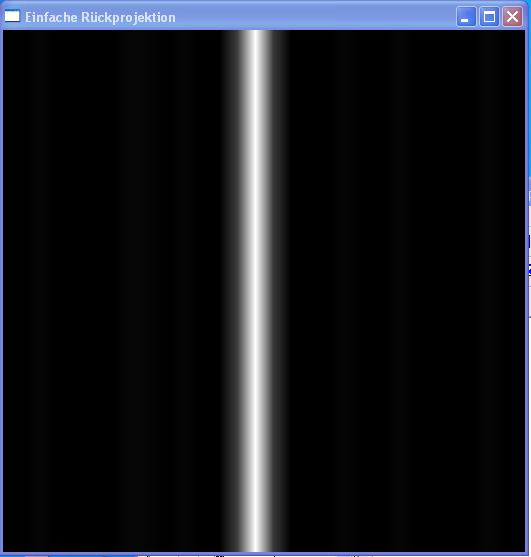
\includegraphics[width=.2\textwidth, height=0.125\textheight]{pic/Einzelfenster_Bilder/inhomogene_Messung/inhomo1einf_prj.png}
                  & 
                  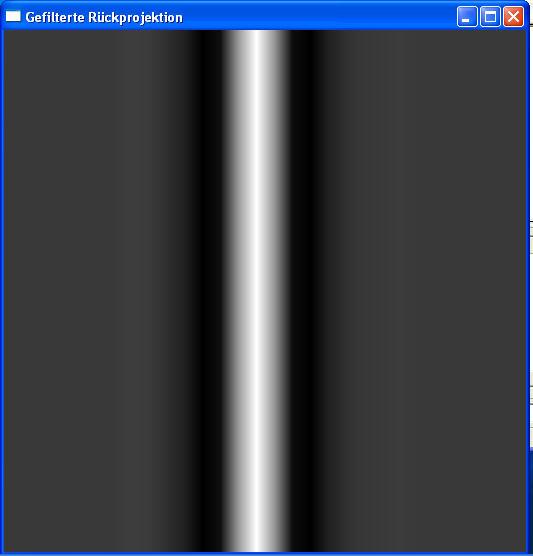
\includegraphics[width=.2\textwidth, height=0.125\textheight]{pic/Einzelfenster_Bilder/inhomogene_Messung/inhomo1gef_prj.png}
                  &
                  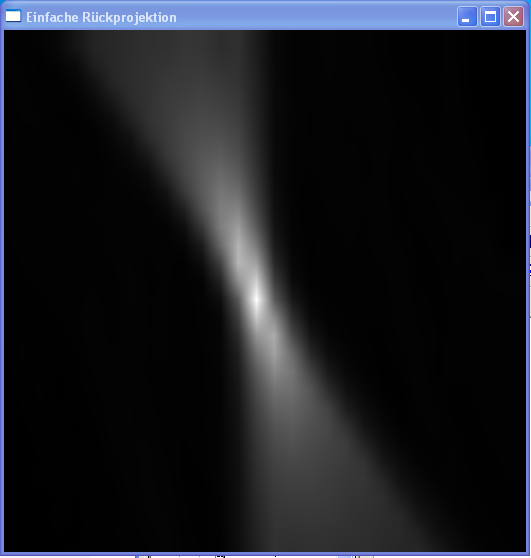
\includegraphics[width=.2\textwidth, height=0.125\textheight]{pic/Einzelfenster_Bilder/isotrope_Messung/iso1einf_rueckprj.png}
                  & 
                  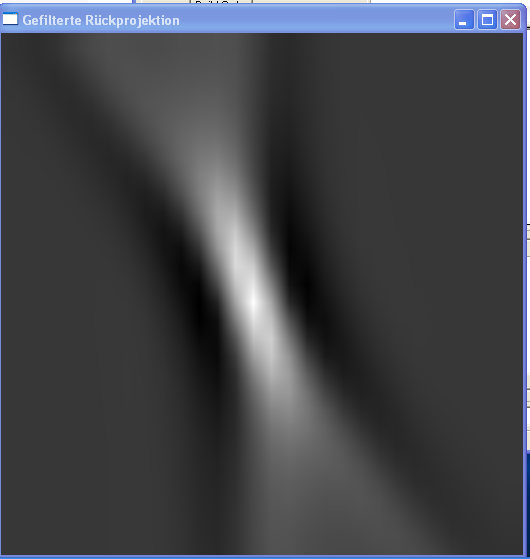
\includegraphics[width=.2\textwidth, height=0.125\textheight]{pic/Einzelfenster_Bilder/isotrope_Messung/iso1gef_prj.png}\\
                  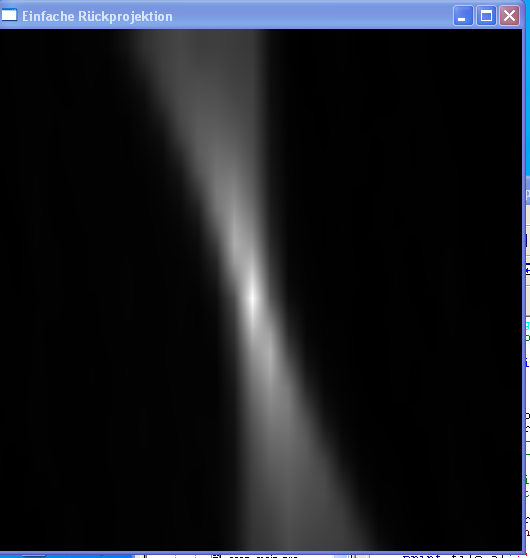
\includegraphics[width=.2\textwidth, height=0.125\textheight]{pic/Einzelfenster_Bilder/inhomogene_Messung/inhomo2einf_rueckprj.png}
                  & 
                  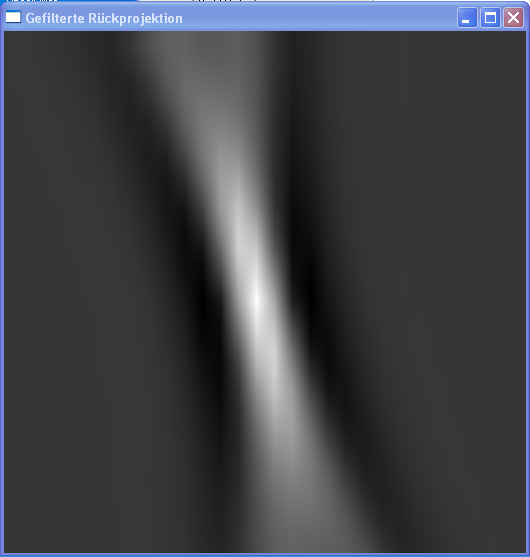
\includegraphics[width=.2\textwidth, height=0.125\textheight]{pic/Einzelfenster_Bilder/inhomogene_Messung/inhomo2gef_prj.png}
                  &
                  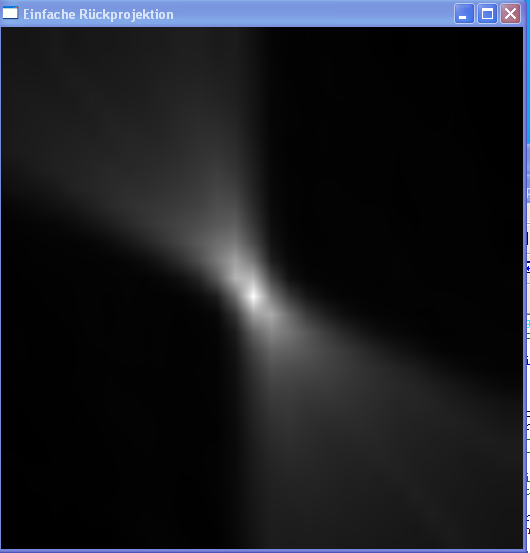
\includegraphics[width=.2\textwidth, height=0.125\textheight]{pic/Einzelfenster_Bilder/isotrope_Messung/iso2einf_rueckprj.png}
                  & 
                  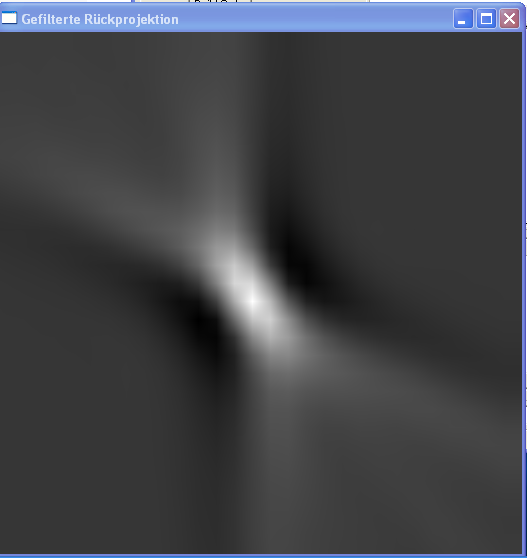
\includegraphics[width=.2\textwidth, height=0.125\textheight]{pic/Einzelfenster_Bilder/isotrope_Messung/iso2gef_prj.png}\\
                  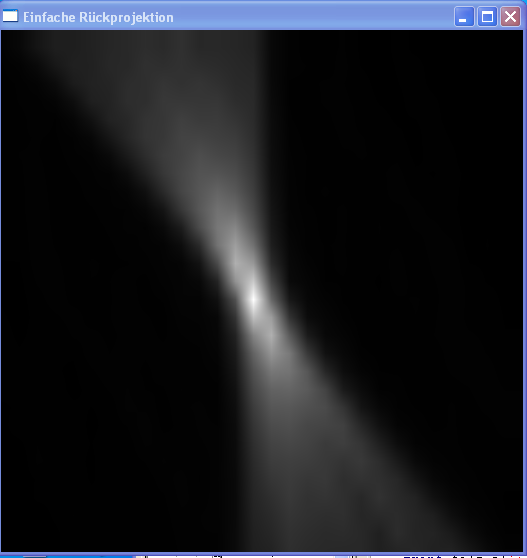
\includegraphics[width=.2\textwidth, height=0.125\textheight]{pic/Einzelfenster_Bilder/inhomogene_Messung/inhomo3einf_rueckprj.png}
                  & 
                  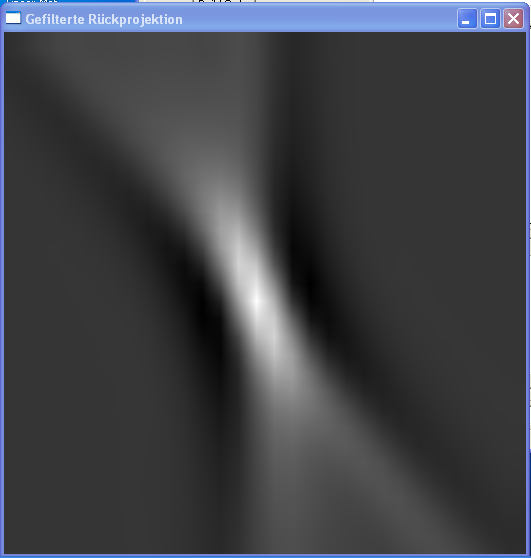
\includegraphics[width=.2\textwidth, height=0.125\textheight]{pic/Einzelfenster_Bilder/inhomogene_Messung/inhomo3gef_prj.png}
                  &
                  \includegraphics[width=.2\textwidth, height=0.125\textheight]{pic/Einzelfenster_Bilder/isotrope_Messung/iso3einf_rueckprj.png}
                  & 
                  \includegraphics[width=.2\textwidth, height=0.125\textheight]{pic/Einzelfenster_Bilder/isotrope_Messung/iso3gef_prj.png}\\
                  \includegraphics[width=.2\textwidth, height=0.125\textheight]{pic/Einzelfenster_Bilder/inhomogene_Messung/inhomo4einf_rueckprj.png}
                  & 
                  \includegraphics[width=.2\textwidth, height=0.125\textheight]{pic/Einzelfenster_Bilder/inhomogene_Messung/inhomo4gef_prj.png}
                  &
                  \includegraphics[width=.2\textwidth, height=0.125\textheight]{pic/Einzelfenster_Bilder/isotrope_Messung/iso4einf_prj.png}
                  & 
                  \includegraphics[width=.2\textwidth, height=0.125\textheight]{pic/Einzelfenster_Bilder/isotrope_Messung/iso4gef_prj.png}\\
                  \includegraphics[width=.2\textwidth, height=0.125\textheight]{pic/Einzelfenster_Bilder/inhomogene_Messung/inhomo5einf_rueckprj.png}
                  & 
                  \includegraphics[width=.2\textwidth, height=0.125\textheight]{pic/Einzelfenster_Bilder/inhomogene_Messung/inhomo5gef_prj.png}
                  &
                  \includegraphics[width=.2\textwidth, height=0.125\textheight]{pic/Einzelfenster_Bilder/isotrope_Messung/iso6einf_prj.png}
                  & 
                  \includegraphics[width=.2\textwidth, height=0.125\textheight]{pic/Einzelfenster_Bilder/isotrope_Messung/iso6gef_prj.png}\\
                  \multicolumn{2}{c}{\includegraphics[width=.2\textwidth, height=0.25\textheight]{pic/Einzelfenster_Bilder/inhomogene_Messung/inhomo5sino.png}}
                  &
                  \multicolumn{2}{c}{\includegraphics[width=.2\textwidth, height=0.25\textheight]{pic/Einzelfenster_Bilder/isotrope_Messung/iso6sino.png}}
           \end{longtable}
           \ \\
           Demgegenüber stehen die Bilder der anisotropen Messung. Man erkennt hier in der Mitte des Sinogramms eine dunklere Stelle und in den abgeschlossenen Rückprojektionen sieht man rechts und
           linksdunklere Stellen, die das Halo unterbrechen. Uns wurde bekanntgegeben, dass nur auf einer Seite eine Anisotropie eingesetzt wurde. Wir sehen diese Unterbrechung jedoch sowohl links als 
           auch rechts. Das bedeutet, dass man in der Praxis nicht mit Sicherheit sagen, wo sich ein festerer Stoff wie zum Beispiel ein Knochen befindet.\\ \ \\
        
        \textbf{Gegenüberstellung der registrierten Ereigniszahlen und Ermittlung einer Korrekturfunktion}\\
        Als nächstes schaut man sich die registrierten und auch tatsächlich für die Rückprojektion verwendeten Ereignisdaten an. Zunächst folgt in Abbildung \ref{dfd:iso} die Darstellung der Ereignisszahlen
        über den Winkel. Man sieht, wie sich die Werte um eine gedachte, konstante Linie herum verteilen und damit die Isotropie. In der nachfolgenden Abbildung \ref{dfd:aniso} sieht man im Gegenteil dazu 
        deutlich die Anisotropie, gekennzeichnet durch eine Mulde, die demnach auszeichnet, dass die Dichte des Materials hier größer war, da weniger Ereignisse gezählt werden. 
        
        \centering \includegraphics[width=.72\textwidth, height=0.225\textheight]{pic/isotropie.png}
        \captionof{figure}{Plot der registrierten Ereigniszahlen}
        \label{dfd:iso}
        \centering \includegraphics[width=.75\textwidth, height=0.25\textheight]{pic/KorrekturderAnisotropie.png}
        \captionof{figure}{registrierte Ereignisse (gelb), korrigierte Ereigniszahlen (schwarz) und Korrekturfunktion (blau)}
        \label{dfd:aniso}
        \flushleft
        Diese Mulde, die wie eine Art Tal irgendwie gaußförmig aussieht, kann man durch eine Korrekturfunktion auf das konstante Niveau anheben. So hat jedes Material seine eigene Korrekturfunktion.
        In Abbildung \ref{dfd:aniso} erkennt man, dass die schwarze Kurve wieder ungefähr um eine konstante Kurve verteilt.
        Die Korrekturfunktion und insbesondere ihre Parameter sind durch ausprobieren entstanden. Die Funktion sieht folgendermaßen aus: 
        \begin{equation*}
            K(\theta) = \frac{A}{\sqrt{2\pi}\sigma} e^{-\frac{1}{2}\left(\frac{\theta - \Delta \theta}{\sigma}\right)^2} \text{ mit folgenden Parametern } \sigma=\unit[14]{°}, A=\unit[1300]{°} \text{ und } \Delta \theta = \unit[98]{°}
        \end{equation*}
        
        